% class
\documentclass{report}

% packages
\usepackage[utf8]{inputenc}
\usepackage{listings}
\usepackage[english, italian]{babel}
\usepackage{graphicx}
\usepackage{algorithm} % package : texlive-science
\usepackage[noend]{algpseudocode}


% custom configurations
%% custom ToC name
\lstset{basicstyle=\footnotesize\ttfamily,breaklines=true,frame=single}
\addto\captionsitalian{
	\renewcommand{\contentsname}
	{Indice}
}

\title{Reti di Elaboratori}
\author{Davide Pucci \& Marco Panunzio}
\date{2016}

\begin{document}

\maketitle

\tableofcontents

\chapter{Introduzione}
\section{Note del corso}
Il corso di Reti di Elaboratori segue i capitoli del Kurose-Ross.
I tre macro-argomenti sono:
\begin{enumerate}
  \item Fondamenti di fisica
  \item TCP/IP
  \item Reti wireless, sicurezza delle reti, e così via \ldots
\end{enumerate}

\section{Componenti della rete Internet}
Centinaia di milioni di dispositivi (\textbf{hosts} o endsystems) che ospitano \textbf{network apps} sono interconnessi insieme ai router tramite \textit{connection links}. 

\begin{itemize}
    \item
        \textit{Hosts} (o \textit{End-Systems}), sui quali girano applicazioni web. \textit{End Systems} perché sono le foglie di un albero di collegamenti che passano per diversi \textit{router} (i quali permettono lo scambio di informazioni tra i vari hosts);
    \item
        \textit{Communication Links} (fibra, radio, satellite, e così via \ldots), a cui è associato un determinato insieme di frequenze, detto \textit{banda}. Conoscendo la banda è possibile ricavare il quantitativo di bit massimo che posso far attraversare, il \textit{datarate} (o \textit{tasso di trasmissione}). La \textit{collisione} è la sovrapposizione di pacchetti di comunicazione da sorgenti diverse, e causa la mancata decodifica dei pacchetti da parte del router;
    \item
        \textit{router} è l'elemento cui viene affidato il compito di gestire l'inoltro dei pacchetti dalla sorgente alla destinazione. È formato da link di ingresso, sui quali esegue il \textit{forwarding} verso i link d'uscita. Per poterlo fare, necessita di un'informazione, l'indirizzo del destinatario. Controlla quindi una \textit{tabella d'inoltro}, composta da due colonne: l'indirizzo del destinatario e \textit{next hop}. Seguendo ogniqualvolta necessario i riferimenti associati all'indirizzo richiesto sulla tabella, il pacchetto arriva a destinazione;
    \item
        \textit{Protocolli} implementano funzionalità necessarie per la rete; controllano la ricezione e la trasmissione di messaggi. Alcuni esempi di protocolli sono TCP, IP, HTTP, ETHERNET e SKYPE.
    \item
        \textit{Standard}: definiscono le regole attraverso cui vengono applicati tutti i protocolli in \textit{internet}.
        \begin{itemize}
            \item L'\textit{RFC} (\textit{request for comments}) contiene tutti gli standard pubblicamente riconosciuti e in vigore su internet.
            \item Lo \textit{IETF} (\textit{internet engineering task force}) viene consultato ogniqualvolta giunge una richiesta di inclusione di un nuovo standard. Dopo essere stato sufficientemente vagliato, lo standard può essere incluso tra gli RFC.
        \end{itemize}
\end{itemize}

\section{Rete Logica e Rete Fisica}
\begin{itemize}
    \item Una \textbf{Rete Fisica} è il diagramma che costituisce l'assetto fisico di una rete. Contiene una serie di nodi - ciascun elemento di rete - legati tra loro da un mezzo trasmissivo;
    \item Una \textbf{Rete Logica} è il diagramma che costituisce l'assetto logico di una rete. Partendo da quello fisico, in questo caso, per ogni nodo possono essere applicate delle policies che permettono - o meno - la trasmissione di dati attraverso mezzi trasmissivi, verso un dato elemento di rete ad esso fisicamente collegato.
\end{itemize}

\section{Internet: Servizi di comunicazione}
I protocolli definiscono come avvengono i colloqui tra dispositivi attraverso specifici set di regole.

\subsection{TCP}
Il \textit{Transmission Control Protocol} è un protocollo di rete che si occupa di rendere affidabile la trasmissione dati in rete tra mittente e destinatario.
In particolare, questo protocollo fornisce:
    \begin{itemize}
        \item trasferimento dati ordinato e affidabile: permette riconoscimento e ritrasmissione di eventuali perdite di dati
        \item controllo del flusso: il mittente non sovraccaricherà il ricevente
        \item controllo della congestione: il mittente rallenterà la velocità di invio quando la rete è congestionata
    \end{itemize}

    \subsubsection{Handshake}
    Si definisce \textit{handshake} (lett. \textit{stretta di mano}) il processo attraverso il quale due calcolatori stabiliscono le regole comuni, ovvero la velocità, i protocolli di compressione, di criptazione, di controllo degli errori etc.
    
    Prima di iniziare la connessione vera e propria tra due macchine si crea questo tipo di connessione che consiste nella trasmissione dei pacchetti per regolare i parametri di connessione.

\subsection{UDP}
Lo \textit{User Datagram Protocol}, a differenza del protocollo TCP non esegue alcun tipo di \textit{handshake} o controllo: questo è utile (o necessario) per alcuni tipi di applicativi che fanno loro componente fondamentale la rapidità di trasmissione di dati, come i servizi di streaming o voip, per i quali diventa di fondamentale importanza la rapidità di ricezione dei pacchetti, piuttosto che la loro qualità.

\section{Trasmissione Dati}
\begin{itemize}
    \item \textbf{Commutazione di Circuito}: si stabilisce un circuito (percorso) tra mittente e destinatario, soltanto dopo aver appurato che le risorse necessarie per effettuare l'effettiva trasmissione dei dati siano disponibili.
    Qualora ci fossero diversi utenti, la suddivisione delle risorse potrebbe avvenire attraverso due modalità:
    \begin{itemize}
        \item \textbf{FDM}: \textit{Frequence Division Multiplexing}, che consiste nel suddividere le risorse in canali, uno per utente. In questo modo ogni utente avrà 1/x delle risorse totali a propria disposizione, dove x è il numero di utenti che utilizza la rete;
        \item \textbf{TDM}: \textit{Time Division Multiplexing}, che consiste nel suddividere le risorse in base al tempo. Ogni utente utilizza la totalità delle risorse disponibili per un determinato lasso di tempo, a conclusione del quale l'utilizzo delle risorse passa all'utente successivo fino a ricominciare il ciclo con il primo utente.
    \end{itemize}
    \textbf{ESEMPIO}. Vogliamo ricavarci il tempo necessario per trasmettere 640.000 bit da un host A ad un host B, sapendo che la rete ha una banda di 1,536Mbps.
    \begin{equation}
        1,536/24 = 64K \to 64.000/640.000 = 1/10s
    \end{equation}
    \textbf{ESEMPIO}. Trasmettiamo 7,5Mbit con una banda massima di 1,5Mbps.
    \begin{equation}
        3*7,5/1,5 = 3*5 = 15s
    \end{equation}
    \newpage
    
    \item \textbf{Commutazione di Pacchetto}: ogni informazione da trasmettere viene suddivisa in \textit{n} pacchetti. Ogni host condivide in questo caso le stesse risorse di rete, ogni pacchetto utilizza tutta la banda disponibile e le risorse vengono adoperate soltanto quando necessario.
    Solitamente le code di pacchetti sono gestite in ordine di arrivo. \\ \\
    \textbf{ESEMPIO}. Trasmettiamo 7,5Mbit con una banda massima di 1,5Mbps.
    \begin{enumerate}
        \item Dividiamo l'informazione da trasmettere in 5000 pacchetti da 1500 bit;
        \item Occorre quindi 1ms per trasmettere pacchetti su un link
        \item Ogni link lavora in parallelo (\textit{pipelining})
        \item Il delay è ridotto da 15s (nel caso dello stesso esempio applicato in un paradigma a commutazione di circuito) a 5,003s.
    \end{enumerate}
\end{itemize}
Il paradigma a commutazione di pacchetto permette a più utenti di utilizzare - in tutta la sua banda e potenza - la stessa rete.

\section{Tipi di Sorgenti}
Le sorgenti di trasmissione dei dati possono utilizzare tassi di frequenza di trasmissione diversi:
\begin{itemize}
    \item \textbf{Tasso costante}: nel caso della telefonia, per esempio, i pacchetti hanno una dimensione fissa e vengono trasmessi ad intervalli regolari. La frequenza è di 64Kbps;
    \item \textbf{Tasso variabile}: facendo riferimento all'esempio precedente, alcuni software gestiscono in maniera ottimale la trasmissione dei dati: associaziono ad una variabile il rumore di sottofondo. Ogniqualvolta riconosceranno - utilizzando quella variabile - che l'utente non sta parlando, non invieranno alcun pacchetto.
\end{itemize}

\section{Network Edge}
Come già anticipato, ogni \textit{end-system} (\textit{host}) esegue applicativi. Questo può avvenire secondo diverse modalità:
\begin{itemize}
	\item \textbf{Client-Server}: un host (\textit{server}) esegue applicativi adibiti alla manipolazione di informazioni, ma soprattutto allo scambio di informazioni con altri host (\textit{client}). Quindi, essenzialmente, i \textit{client} effettuano richieste ai \textit{server}, che eseguono servizi perennemente in esecuzione (\textit{always-on});
	\item \textbf{Peer-Peer}: non esiste differenziazione tra \textit{server} e \textit{client}, perché in questo caso gli host eseguono le stesse attività, ma comunicando tra loro (come nei casi di servizi come \textit{Torrent}, \textit{Skype}, e così via \ldots).
\end{itemize}

\section{Accesso alla rete}
Ogni dispositivo può essere connesso ad internet tramite diverse \textit{reti di accesso}. Possono essere:
\begin{itemize}
	\item Reti residenziali
	\item Reti istituzionali (scuole, aziende, e così via \ldots)
	\item Reti mobili (come quelle utilizzate dagli smartphones)
\end{itemize}
Elementi essenziali della rete di accesso sono la banda (bit/s), l'affidabilità (bit error rates) e se è dedicata o condivisa.
\paragraph{Punti di accesso mobili}
Un altro elemento fondamentale è il punto di accesso alla rete: essa dev'essere in grado di riconoscere che si sta degradando il segnale e individuare un altro punto di accesso al quale ci stiamo avvicinando, così da evitare un'eventuale degradazione della qualità della rete quando si è in movimento.

\section{Trasmissione attraverso link fisici}
Ciò che viene trasmesso è una sequenza di bit che codifica il contenuto.
\begin{itemize}
	\item \textbf{Bit}: valori che si propagano tra il trasmettitore e il ricevitore
	\item \textbf{Link}: tracce attraverso cui passano i bit
	\begin{itemize}
		\item \textbf{Tracce guidate}: cavi fisici (fibra, e così via \ldots)
		\item \textbf{Tracce radio}: le informazioni vengono trasmesse attraverso onde radio
	\end{itemize}
\end{itemize}

Le informazioni trasmesse tramite onde radio subiscono un'\textit{attenuazione} durante la propagazione dell'informazione, e quindi una \textit{distorsione}.
Ciò non avviene in maniera uniforme; bisogna anche mettere in conto eventuali interferenze elettromagnetiche (spesso introdotte dalle stesse apparecchiature utilizzate per la connessione). Il risultato è che la sequenza ricevuta potrebbe non essere corretta. Questo introduce la definizione di \textit{bit error rate}, ovvero la frequenza con cui si verifica un errore nella trasmissione delle informazioni. Minore è il suo valore, migliore e più stabile è la rete.
In questo caso, occorre che il dispositivo sia \textit{error-aware}, così da essere autonomo nell'individuare la presenza di errori e tentare di correggerli (possibile fino a un certo numero di bit, altrimenti viene scartato il pacchetto e richiesto indietro).

\subsection{Codifica NRZ}
\textit{NRZ: Non Return to Zero}. Il tempo è diviso in slot - unità temporali che corrispondono ad un bit.
Ogni bit ha associato un valore stabile per la sua intera durata (1: High, 0: Low).
Il problema in questo tipo di codifica è la spesso asicronizzazione tra trasmettitore e ricevitre.

\subsection{Codifica Manchester}
Utilizzata in Ethernet. Essenzialmente viene associato un valore ad ogni transizione. Quando la frequenza di trasmissione va dal basso all'alto - di intensità - il valore associato è 1, dall'alto al basso, invece, 0.

\section{Tecnologie di accesso}
\subsection{Dial-up modem}
Velocità trasmissiva: 56Kbps (ca.). Utilizza la stessa infrastruttura telefonica: non \textit{always-on}, impossibile poter usufruire della linea per internet e telefonia allo stesso tempo.
Il modem reindirizza le richieste al \textit{central office}, che - qualora si cerchi di navigare in internet - converte la richiesta e la reindirizza all'\textit{ISP} (\textit{Internet Service Provider}).

\subsection{Digital Subscriber Line}
Anch'essa utilizza un'infrastruttura telefonica esistente. Spesso chiamata anche A-DSL (la \textit{A} indica l'\textit{asimmetria} tra la velocità di trasmissione modem-\textit{central office} e \textit{central office}-modem).
Essendo la frequenza del segnale vocale sempre in un intervallo tra 0 e 4KHz, il segnale può essere campionato fino a 8M volt/s ed essere successivamente ricostruito; in quella frequenza il segnale è trasmesso \textit{solo} attraverso via telefonica. Tutte le trasmissioni fuori da quell'intervallo vengono quindi campionate come richieste per internet.
Le risorse del canale sono divise attraverso \textit{FDM} (\textit{Frequency Division Multiplexing}).\\
Velocità: fino a 1Mbps up (tipicamente $<$ 256Kbps) e a 8Mbps down (tipicamente $<$ 1Mbps) down. La grande differenza di velocità trasmissiva è causata da un paradigma client/server che dà la precedenza al download dei dati piuttosto che alla loro trasmissione.
\\
Tecnologie di tipo DSL sono progettate per raggiungere distanze non molto elevate (fino a 4/5 km).
\paragraph{ADSL loop extender} 
Dispositivo posizionato tra il cliente e il central office dalla compagnia telefonica per estendere la distanza ed aumentare la velocità di trasmissione.

\subsection{HFC (in \textit{USA})}
Velocità: fino a 20Mbps down, 2Mbps up.
Utilizza - invece dell'infrastruttura telefonica - quella della TV via cavo.
Sostanzialmente il \textit{central office}, in questo caso il \textit{cable headend}, gestisce degli anelli di fibra, composti da moltissimi nodi che li collegano ad ogni abitazione. A questo punto, la connessione passa per uno splitter (che utilizza l'\textit{FDM}), che la indirizza alla TV o al dispositivo che richiede la connessione internet. 

\subsection{Fibra ottica}
Collegamenti ottici dal \textit{central office} all'abitazione. Raggiunge distanze lunghissime praticamente senza alcuna distorsione del segnale.
Due tipologie di accesso:
\begin{itemize}
	\item \textit{Passive Optical Network} (\textit{PON}): un'unica fibra e uno splitter ottico che smista le informazioni verso diverse abitazioni. Comporta costi decisamente bassi, a scompenso però della qualità:
	\begin{itemize}
		\item Si possono spesso verificare \textit{collisioni}, evitate attraverso il \textit{TDM}
		\item Essendo una linea condivisa si presenta la necessità di dover criptare i messaggi
		\item Non raggiunge distanze massime
		\item Diventa più difficile isolare eventuali problemi
		\item Velocità di accesso non ottimale
	\end{itemize}
	\item \textit{Active Optical Network} (\textit{PAN})
\end{itemize}

\subsection{Ethernet}
Evoluzione che risale agli anni '80; tecnologia basata su formati e protocolli che sono rimasti immutati, se non per supportare il decisivo incremento della velocità di navigazione.
Uno switch - con ingressi ethernet, appunto - viene frapposto tra router/modem e diversi host.

\subsection{Wireless Access Networks}
In questo caso, le informazioni sono modulate opportunamente, per raggiungere le frequenze delle onde radio supportate dal ricetrasmettitore radio.
Ne esistono due tipi:
\begin{enumerate}
	\item \textit{Wireless LAN} (o \textit{WiFi}) 802.11b/g: raggiunge una velocità compresa tra gli 11Mbps e i 54Mbps;
	\item \textit{Wide-area Wireless Access}: mezzo radio condiviso che raggiunge una velocità compresa tra 1Mbps (\textit{EVDO}/\textit{HSDPA}) e diverse decine di Mbps (\textit{LTS}).
\end{enumerate}
Essendo la rete condivisa, neccessita di essere criptata. Non utilizza né \textit{FDM} né \textit{TDP}, ma un sistema di gestione proprietario e specifico.

\section{Reti Mobili}
\begin{center}
	\begin{tabular}{| c | c | c | c | c |}
		\hline
		\textbf{Generazione} & \textbf{Simbolgia} & \textbf{Tecnologia } & \textbf{DL Massima} in Mbit/s & \textbf{DL Tipica} in Mbit/s \\ \hline
		2G & G & GPRS & 0,1 & 0,03 \\ \hline
		2G & E & EDGE & 0,3 & 0,1 \\ \hline
		3G & 3G & 3G (basic) & 0,3 & 0,1 \\ \hline
		3G & H & HSPA & 7,2 & 1,5 \\ \hline
		3G & H+ & HSPA+ & 21 & 1 \\ \hline
		3G & H+ & DC-HSPA+ & 42 & 8 \\ \hline
		4G & 4G & LTE & 100 & 15 \\ \hline
	\end{tabular}
\end{center}

\section{Componenti attuali}
\begin{enumerate}
	\item \textit{DSL Fast-Technology} (combinata con fibra): 1Gbps
	\item \textit{Ethernet}: 25-40Gbps (con più linee 100-400Gbps)
	\item \textit{WiFi IEEE 802.11ac}: 1Gbps
	\item \textit{Fibra}: diverse decine di Tbps
	\item \textit{Reti mobili}: diverse centinaia di Mbps
\end{enumerate}

\section{Internet Structure: rete di reti}
Internet ha una struttura gerarchica, composta da moltissimi \textit{ISP} (\textit{Internet Service Provider}).
La prima categoria è composta dai \textit{Tier-1} (Verizon, Sprint, AT\&T, e così via \ldots). Questi sono interconnessi - per maggiore copertura - tramite dei \textit{POP} (\textit{Point of presence}).
Poi ci sono i \textit{Tier-2}, anche loro interconnessi tra loro e con i \textit{Tier-1}.
La gerarchia continua seguendo questo schema, fino a raggiungere gli \textit{ISP} regionali/pronvinciali e, infine, le reti residenziali.
\newpage

\section{Loss \& Delay}
Esistono diversi tipi di ritardi:
\begin{itemize}
	\item \textbf{Processing Delay}: ritardo nel processare i dati ricevuti (per analizzare se contengono errori o meno, per leggere l'header e per instradarli nella coda giusta).
	\item \textbf{Queue Delay}: tempo di attesa prima che il link adibito alla consegna dei dati processi il pacchetto.
	\item \textbf{Transmission Delay}: il tempo necessario a trasmettere tutta la sequenza del pacchetto.
	\begin{itemize}
		\item R = banda link (bps)
		\item L = grandezza pacchetto (bit)
		\item a = frequenza di arrivo pacchetti
		\item \textit{Tempo di trasmissione sul link}: $\frac{L}{R}$
		\item \textit{Intensità di traffico}: $\frac{L\times a}{R}$
	\end{itemize}
	L'arrivo dei pacchetti segue una distribuzione di \textit{Poisson}, e quindi:
	\begin{itemize}
	    \item se l'intensità di traffico è 0 ca., si è verificato un delay piccolo;
	    \item se l'intensità di traffico è 0,5 ca., si è verificato un delay medio;
	    \item se l'intensità di traffico è 1 ca., si è verificato un delay alto e basta pochissimo per congestionare la rete.
	\end{itemize}
	\item \textbf{Propagation Delay}: tempo utilizzato dai bit per propagarsi (alla velocità della luce, ca.) lungo tutta la linea fino alla destinazione.
	\begin{itemize}
		\item d = lunghezza fisica del link
		\item s = tempo di propagazione in media
		\item \textit{Ritardo di propagazione} = $\frac{d}{s}$
	\end{itemize}
	\item \textbf{Nodal delay} = Processing delay + Queue delay + Transmission delay + Propagation delay
\end{itemize}

Il \textit{trace route program} conta il tempo mandando pacchetti con un contatore \textit{time-to-live} che decrementa di 1 all'incrontro con ogni router.
\\
Il \textit{throughput} indica i bit trasmessi al secondo: il collo di bottiglia sarà il link che avrà il \textit{throughput} minore. Viene quindi inviata la massima quantità pari al \textit{throughput} del link più piccolo.

\chapter{TCP/IP}
\section{Protocolli}
\begin{itemize}
    \item \textbf{TCP}: protocollo di trasporto
    \item \textbf{IP}: protocollo di instradamento
\end{itemize}

In una \textit{TCP connection request/response} i protocolli devono specificare:
\begin{itemize}
    \item il formato delle informazioni (ordine dei bit, e quant'altro \ldots)
    \item messaggio da scambiare
    \item ordine degli eventi
\end{itemize}

TCP prevede che prima dello scambio delle informazioni ci sia la \textit{request/response}, un dialogo il cui fine è assicurare che:
\begin{itemize}
    \item i dati siano in ordine e completi
    \item avvenga il \textit{controllo di flusso} (consente di sapere la velocità e la quantità di dati che è possibile trasferire)
    \item avvenga il \textit{controllo di congestione} (i router si accorgono se il flusso in arrivo è maggiore di quello in uscita)
\end{itemize}

A differenza del \textit{TCP}, l'\textit{UDP} non prevede alcuno scambio \textit{request/response}, prima dell'effettivo trasferimento dell'informazione. Il sistema dei \textit{DNS} utilizza \textit{UDP}: quando si ha un \textit{URL}, bisogna ottenerne l'\textit{indirizzo IP} associato, perciò viene richiesta l'informazione tramite il protocollo \textit{UDP}, che garantisce una trasmissione rapida, ma non da certezze che questa vada a buon fine.

\section{Pila TCP/IP}
La \textit{pila TCP/IP} è una pila protocollare, che indica i livelli di protocollo, organizzata a livelli (modularità, così che se variano le regole di un livello, questo cambiamento non tange il funzionamento degli altri).
Tutte le funzionalità logiche si dividono in gruppi, per rendere la progettazione più semplice e più estensibile.
\\
Ciascuna funzionalità ha diversi protocolli.
Il gruppo più in alto corrisponde alla logica applicativa.
Spesso si arricchisce ogni gruppo con microfunzionalità e questo da un servizio aggiuntivo al livello superiore, e queste microfunzionalità possono essere mappate (duplicate) in livelli diversi.
Diverse entità della rete hanno diversi sottoinsiemi delle funzionalità.
Vengono stabiliti gli \textit{access service point} che sono i punti in cui - nell'architettura - c'è il passaggio da un livello ad un altro.
Lo svantaggio di un'architettura di questo tipo è che livelli non adiacenti non hanno la possibilità di comunicare (esiste però un sistema, chiamato \textit{cross layering}, che permette di leggere dati di livelli non adiacenti).
\\
I livelli sono solitamente i seguenti:
\begin{enumerate}
    \item \textbf{Lv "applicativo"} (\textit{software}): molte funzionalità diverse (come la sincronia);
    \item \textbf{Lv di "trasporto"} (\textit{software}): utilizza di base il protocollo \textit{UDP} e controlla che il messaggio venga consegnato al giusto destinatario. Col protocollo \textit{TCP} c'è anche il controllo se il pacchetto è arrivato ed è stato realmente consegnato al giusto destinatario;
    \item \textbf{Lv di "rete"} (\textit{network}): adibito al tentativo di capire il percorso da intraprendere, attraverso algoritmi di instradamenti, per poi inviare il pacchetto attraverso quel percorso;
    \item \textbf{Lv "link"}, o \textbf{datalink} (\textit{hardware}): lavora con i \textit{frame} (\textit{trama}). Verifica se ci sono stati errori di trasmissione, analizzando anche gli indirizzi \textit{MAC} (\textit{Medium Access Control});
    %\item \textbf{Lv "fisico"} (\textit{hardware}): enormi eterogeneità.
\end{enumerate}
Sugli \textit{end-systems} ci saranno tutti e 4 i livelli.
Sugli elementi intermedi di commutazione ci saranno solamente i 3 livelli più bassi.
L'\textit{ack} (\textit{acknowledgement}) è un tipo di messaggio che viene utilizzato per far capire al sorgente/destinatario che il pacchetto è arrivato.
Ogni livello aggiunge un \textit{header}, che per il livello successivo diventa parte integrante del messaggio stesso da consegnare. Per ciascun livello, ecco l'header:
\begin{itemize}
    \item Applicativo: il messaggio stesso (\textit{messaggio}, o \textit{message});
    \item Trasporto: il \textit{segmento}, o \textit{segment};
    \item Rete: il \textit{pacchetto}, o \textit{datagram};
    \item Datalink: la \textit{trama}, o \textit{frame}.
\end{itemize}
I vantaggi della stratificazione sono la modularità e la gestione dell'eterogeneità.

\section{Storia}
Internet è stato inventato da \textit{Leonard Kleinrock}, quand'era ancora studente ed ebbe l'idea dell'architettura a pacchetto, nel 1961.
Nel 1969, 8 anni dopo aver concepito questa idea, viene attivata la prima rete con 4 nodi (le 4 importanti università della California), utilizzando il protocollo \textit{NCP}.
\\
Nel 1972 viene allargata a 15 nodi.
Negli anni successivi altri studenti hanno avuto l'idea di una rete \textit{wireless}, utilzzando il protocollo \textit{ALOHA}, o anche quella di connettere stampanti - o altri dispositivi -, concependo per la prima volta il concetto di \textit{LAN}.
\\
\textit{Robert E. Kahn} e \textit{Vinton Cerf} capirono l'importanza di mantenere l'eterogeneità della rete. Definirono l'architettura di internet odierna.
\\
Così:
\begin{itemize}
    \item 1979: raggiungimento di 200 nodi;
    \item 1982: nasce l'\textit{SMTP} per le email;
    \item 1983: inventato il \textit{TCP/IP};
    \item 1985: nasce l'\textit{FTP} per lo scambio di file;
    \item 1988: viene aggiunto il controllo di congestione al protocollo TCP.
\end{itemize}
Ciononostante, la rete rimaneva una realtà legata all'ambito accademico.
\\
Nei primi anni '90, \textit{Tim Berners-Lee} ebbe l'idea di web così come oggi è conosciuto, inventando l'\textit{HTTP} e l'\textit{HTML}, sulla base di documenti del 1945 di \textit{Vannevar Bush} che accennava agli \textit{ipertesti}.
\\
Da qui in poi internet ha avuto una crescita esponenziale, sia in velocità che in applicazioni.

\chapter{Livello Applicativo}
\section{HTTP}
\section{Cookies}

\chapter{Livello di Trasporto}
\section{Protocolli di Trasporto}
I protocolli di trasporto sono un insieme di protocolli che risiedono sugli host e sugli endsystems; si occupano di fornire le regole per una comunicazione logica tra due entità remote.\\
A livello di invio, si occupano della ricezione dei messaggi in segmenti e li inviano al network layer; alla ricezione, i segmenti sono riassemblati in messaggi e passati al livello applicativo.\\
Mentre il livello di rete offre comunicazione tra due endsystems (trasportando informazioni da un host all'altro), il livello di trasporto crea un collegamento logico tra due \textit{processi}. Deve quindi essere in grado di raccogliere flussi informativi, utilizzare il livello di rete per trasportarli e successivamente smistarli nei vari processi applicativi.

\section{Internet transport-layer protocols}
A dispetto del fatto che il livello rete utilizza una best-effort policy che non dà nessuna garanzia di consegna, \textbf{TCP} si occuperà di applicare meccanismi per la traduzione di informazioni agli opportuni processi anche nel caso di perdita di dati.\\
I principali tipi di perdita dei dati sono:
\begin{itemize}
	\item un eccesso di informazioni arrivate al router intermedio. \\
	La conseguenza è un riempimento delle code fino al raggiungimento di una congestione in rete e all'inizio di una perdita di pacchetti.
	\item il ricevimento a destinazione di un tasso di informazioni troppo elevato rispetto alla velocità di lettura. \\
\end{itemize}
Si noti che un controllo del flusso di informazioni richiede algoritmi diversi rispetto al controllo di congestione; entrambi i tipi di controllo sono implementati da TCP.

\section{Multiplexing e Demultiplexing}
L'invio di informazioni da parte di un processo è eseguito attraverso una determinata porta dotata di interfacce ben definite. Tale porta, che consente il colloqui con l'entità sottostante di livello trasporto, prende il nome di \textit{socket}.\\
Poiché più flussi informativi sono trasmessi tramite lo stesso canale logico, occorre stabilire delle funzioni di smistamento di dati. Queste funzioni sono implementate nei protocolli TCP e UDP in maniera differente.\\

\subsection{UDP: Connectionless demux}
Il socket creato è dotato di un numero di porta dell'host locale; quando viene creato un \textit{datagram} (pacchetto) da inviare nel socket UDP, questo deve specificare l'indirizzo IP e il numero di porta dell'host di destinazione.
Quando l'host remoto riceve un segmento via UDP, controlla il suo numero di porta di destinazione e lo indirizza alla porta corrispondente.
Pacchetti con stesso numero di porta di destinazione, ma indirizzi IP o porte di origine differenti saranno quindi orientati allo stesso socket a destinazione.

\section{TCP: Connection-oriented demux}
In questo caso viene creato un socket dedicato al flusso di informazioni identificato dalla presenza di quattro campi: due per gli indirizzi IP del mittente e del destinatario, due per i numeri di porta del mittente e del destinatario.
Nel caso di più client connessi allo stesso webserver, all'inizio viene fatta una richiesta su un \textit{welcome-socket} generale; successivamente le richieste sono smistate ad un socket dedicato su ciascuna delle connessioni: in questo modo è assicurato che il flusso di dati passerà per socket differenti.
\newpage

\section{Reliable Data Transfer}
La necessità di strutturare un protocollo di trasferimento di dati affidabile nasce dall'importanza che due entità, in comunicazione, siano in equilibrio in termini di velocità di produzione/trasmissione/consumo dei dati, senza che l'eventuale fallimento nella trasmissione tramite livelli inferiori - nella pila TCP/IP - causi il definitivo fallimento della trasmissione. \\
Sarà fatto uso della rappresentazione FSM, una tipologia di rappresentazione utile alla sintetizzazione grafica dei servizi orientati alla connessione.
\begin{center}
    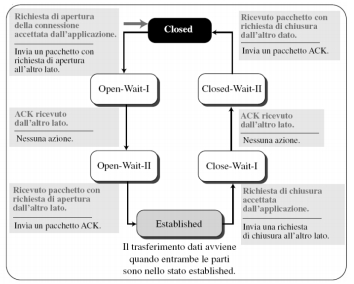
\includegraphics[width=.7\textwidth]{res/fsm.jpg} \hfill
\end{center}

\subsection{RDT 1.0}
Il caso riguardante \textit{RDT 1.0} è contestualizzato in una situazione perfettamente affidabile:
\begin{itemize}
    \item non si verificano \textbf{mai} errori nei bit trasmessi;
    \item non si verifica \textbf{mai} una perdita di pacchetti.
\end{itemize}
\begin{center}
    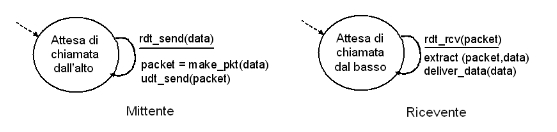
\includegraphics[width=.7\textwidth]{res/fsm-rdt-10.jpg} \hfill
\end{center}
\newpage

\subsection{RDT 2.0}
In questo caso, il canale di trasmissione effettiva può confondere i bit nel pacchetto. Da qui la necessità di introdurre dei messaggi di risposta alla ricezione di un pacchetto:
\begin{itemize}
    \item \textbf{ACK} (\textit{ACKnowledgment}, o \textit{conferma di ricezione}): utilizzato per confermare che il pacchetto è stato ricevuto ed è integro;
    \item \textbf{NAK} (\textit{Negative AcKnowledgment}, o \textit{conferma negativa}): il pacchetto contiene errori. Il mittente reinvia il pacchetto quando riceve indietro questo tipo di messaggio: motivo per cui si tratta di un protocollo \textit{ARQ} (\textit{Automatic Repeat reQuest}, o \textit{Richiesta Automatica di Ripetizione}.
\end{itemize}
\begin{center}
    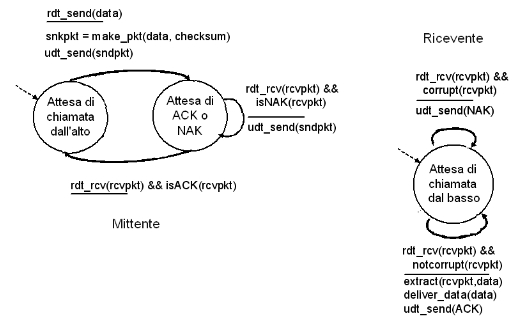
\includegraphics[width=.7\textwidth]{res/fsm-rdt-20.jpg} \hfill
\end{center}
\textit{RDT 2.0} può però andare incontro ad un difetto fatale: la mancata gestione degli eventi in cui i pacchetti \textit{ACK}/\textit{NAK} siano danneggiati.

\subsection{RDT 2.1}
Viene dunque aggiunto - alternativamente - un valore binario a ciascun pacchetto, un \textit{numero di sequenza}.
In questo modo, viene comunicato non solo l'esito della ricezione al mittente, ma anche il pacchetto a cui questo fa riferimento. \\
\begin{minipage}[t]{0.5\textwidth}
    \begin{center}
        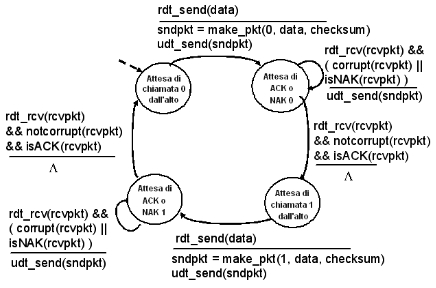
\includegraphics[width=.8\textwidth]{res/fsm-rdt-21-sender.jpg} \hfill
    \end{center}
\end{minipage}
\begin{minipage}[t]{0.5\textwidth}
    \begin{center}
        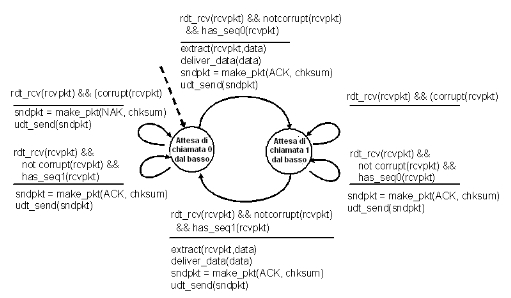
\includegraphics[width=.8\textwidth]{res/fsm-rdt-21-receiver.jpg} \hfill
    \end{center}
\end{minipage}
\newpage

\subsection{RDT 2.2}
\textit{RDT 2.2} fornisce le stesse funzionalità di \textit{RDT 2.1}, utilizzando però soltanto gli \textit{ACK}, escludendo i \textit{NAK}.
Nel caso in cui il destinatario dovesse inviare un \textit{NAK}, invia nuovamente un \textit{ACK} con numero di sequenza dell'ultimo pacchetto ricevuto correttamente.
\begin{center}
    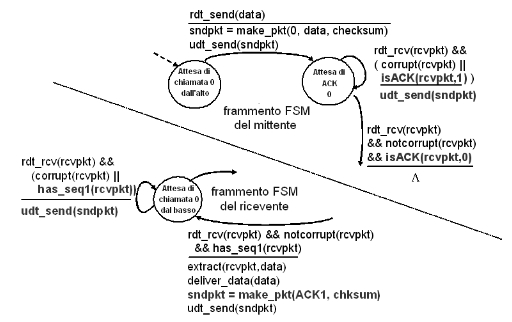
\includegraphics[width=.7\textwidth]{res/fsm-rdt-22.jpg} \hfill
\end{center}

\subsection{RDT 3.0}
L'alternativa è invece introdurre una nuova funzione di timing. Per ogni pacchetto inviato, il mittente implementa un timer: una volta che questo raggiunge un timeout, se non ha ricevuto nessun pacchetto che gli comunichi l'esito (l'\textit{ACK}), allora reinvia il pacchetto. Per questo motivo:
\begin{itemize}
    \item il mittente deve tenere una copia del pacchetto spedito fino a che non ne riceve riscontro dell'esito;
    \item per garantire il controllo di flusso, non si spedisce più di un pacchetto alla volta.
\end{itemize}
Il parametro \textit{RTT} (o \textit{Round Trip Time}) viene definito come il tempo necessario per l'invio di un pacchetto sommato a quello per la ricezione di un pacchetto riferito all'esito del precedente.
\paragraph{Esempio.}
In un link da 1Gbps, con un \textit{propagation delay} di 15ms e 8000bit per ciascun pacchetto abbiamo:
\begin{center}
$ D = \frac{L}{R} = \frac{8000bit}{10^9 bit/s} = 8microsecs $ \\
$ U = \frac{\frac{L}{R}}{RTT + \frac{L}{R}} = \frac{0,0008}{30,0008} = 0,00027 $
\end{center}
\newpage

\subsection{Protocolli a Ritrasmissione Automatica (o \textit{a finetra})}
A differenza dei precedenti, viene trasmessa sempre una sequenza di pacchetti. A man mano che si ricevono gli ACK, vengono aggiunti nuovi pacchtti in coda.
In questo caso: $ U = \frac{\frac{3L}{R}}{RTT + \frac{L}{R}} $ \\
\paragraph{Go-back-N.} Il mittente può avere fino a N pacchetti non riconosciuti nella pipeline. Il destinatario invia solo \textit{ACK cumulativi}, ovvero relativi ad un gruppo di pacchetti ricevuti. Il mittente utilizza un timer per legato al primo pacchetto inviato che ancora non ha ricevuto ACK: al suo raggiungimento, reinvia tutti i pacchetti a partire da quello per il quale ha impostato il timeout.
\paragraph{Selective Repeat.} Il mittente può avere fino a N pacchetti. Il destinatario invia un \textit{ACK individuae}, relativo quindi ad ogni pacchetto. Il mittente utilizza invece un timer per ogni pacchetto di cui non ha ricevuto esito; quando raggiunge il timeout, ritrasmette solo quel dato pacchetto.

\section{Ritrasmissione Automatica in TCP}
TCP utilizza una versione ibrida dei protocolli \textit{Go-back-N} e \textit{Selective repeat}: invia un flusso di singoli bytes che formano - per mano del ricevente - un segmento, il cui \textit{sequence number} è quello del primo byte contenuto, e la cui lunghezza è determinata dal numero totale di bytes. Utilizza inoltre una variabile definita come \textit{MSS}, che indica la lunghezza massima di ciascun segmento. \\
In una stessa connessione, il flusso di dati è bidirezionale, viene eseguito un \textit{handshake} per inizializzare i buffer e alcune variabili (come la \textit{MSS} stessa). La dimensione dei buffer varia nel tempo, sulla base delle informazioni raccolte dai controlli di flusso e congestione. \\
Ogni segmento è composto dai seguenti campi (ciascuno da 32bit):
\begin{itemize}
	\item Porta sorgente / destinazione;
	\item \textit{Sequence number};
	\item \textit{Acknowledgment number}: eventuale ACK di riscontro per un pacchetto appena ricevuto (necessario perché la connessione è bidirezionale);
	\item \textit{Checksum};
	\item \textit{Header length}: se si desidera aggiungere informazioni addizionali, è necessario specificarne la lunghezza;
	\item \textit{Receive window}: indica quanto spazio ho ancora nel buffer (necessario per la gestione del flusso);
	\item \textit{RST}/\textit{SYN}/\textit{PIN}: variabili settate a \textit{1} in fase di apertura/chiusura della connessione;
	\item \textit{ACK}: variabile settata a \textit{1} se il ricevente deve leggere il campo \textit{Acknowledgment number};
	\item \textit{URG}: indica che si tratta di un pacchetto più urgente della media;
	\item \textit{Application Data}: dati da trasmettere.
\end{itemize}

\subsection{Meccanismi di controllo affidabile}
In \textit{TCP} - lato \textit{sender} - viene, per ciascuna connessione e trasmissione, creato un segmento con \textit{numero di sequenza} \textit{n}, che corrisponde al primo byte del flusso di bytes in trasmissione attraverso quello stesso segmento. \\
Se un timer è già attivo, rimane invariato, perché ancora non è stato ricevuto riscontro su una serie di segmenti; altrimenti, lo avvio. \\
Al timeout, ritrasmesso il primo segmento che lo ha causato, ma non tutto, perché \textit{TCP} permette l'inserimento dei buffer contenenti i flussi di bytes ricevuti non necessariamente in sequenza per conservarli. Poi viene riavviato il timer. \\
Al ricevimento dell'\textit{ACK}, si controlla se è relativo ad un segmento di cui non si conosce l'esito di ricezione:
\begin{enumerate}
    \item applico l'\textit{ACK} a tutti i segmenti di cui non avevo ancora ricevuto l'esito fino a quest'ultima ricezione;
    \item avvio un nuovo timer.
\end{enumerate}

\subsection{Variabilità del retransmission timeout}
Ovviamente, il timeout deve essere necessariamente $/geq RTT$ (\textit{RoundTrip Time}). Inoltre:
\begin{itemize}
    \item se troppo corto, avvengono ritrasmissioni inutili e non necessarie;
    \item se troppo lungo, i tempi di reazione diventano troppo lunghi se i segmenti sono andati perduti.
\end{itemize}
Per ovviare a questi problemi, è stato introdotto una stima calcolata per ottenere dinamicamente un timeout più adatto alle prestazioni di rete di ciascuna connessione. Viene utilizzato un \textit{SampleRTT}, ovvero l'\textit{RTT} dell'ultima trasmissione eseguita della quale è stato ricevuto l'\textit{ACK}. A questo punto viene utilizzata una media esponenziale pesata per tenere in conto della variabilità nel tempo dei vari \textit{SampleRTT}, nella cui formula viene utilizzata una variabile $\alpha$, tipicamente impostata a \textit{0,125}, la cui funzione è quella di dare maggiore importanza ai \textit{SampleRTT} più recenti, rispetto che a quelli più lontani nel tempo. Il risultato è la seguente formula: \\
\begin{center}
    $ EstimatedRTT = (1-\alpha )\times EstimatedRTT + \alpha \times SampleRTT $
\end{center}
A questo punto, questa stima viene utilizzata nel calcolo della deviazione dell'\textit{RTT}, in cui compare una nuova variabile $\beta$, la cui funzione è identica a quella della variabile $\alpha$ vista in precedenza, ma che è tipicamente valutata \textit{0,25}: \\
\begin{center}
    $ DevRTT = (1-\beta )\times DevRTT + \beta \times \left| SampleRTT - EstimatedRTT \right| $
\end{center}
Infine, il valore del timeout stimato come migliore possibile ed effettivamente utilizzato:
\begin{center}
    $ Timeout = EstimatedRTT + 4 \times DevRTT $ \\
\end{center}

\subsection{Controllo del flusso}
Il \textit{Flow Control} è utilizzato per evitare di saturare il \textit{buffer} dentro cui vengono conservati i pacchetti ricevuti, prima che vengano prelevati dal \textit{layer applicativo}. Se questo venisse riempito troppo rapidamente, rispetto alla velocità di prelevamento dei dati, ci si troverebbe in una situazione di criticità. \\
Per questa ragione, vengono segnalate al \textit{sender} informazioni sullo spazio a disposizione, nel campo \textit{receive window} (da \textit{16bit}) nel segmento: il \textit{sender} adegua il flusso dei dati trasmesso di conseguenza. \\
La \textit{finestra} e il \textit{buffer} sono configurati nell'\textit{handshake} della connessione, tramite i campi:
\begin{itemize}
    \item \textbf{MSS} (\textit{Maximum Sequence Size}): impostato tipicamente a 2K, indica la lunghezza massima del segmento;
    \item \textbf{ISN} (\textit{Initial Sequence Number)}: impostato tipicamente a 2047 (e chiaramente variando in base al valore del \textit{MSS}), indica il valore iniziale del \textit{sequence number};
    \item \textbf{WIN} (\textit{WINdow}): impostato tipicamente a 4K, indica la dimensione della finestra.
\end{itemize}
Ad ogni trasmissione, viene specificato anche il valore \textit{WIN} sulla base dello spazio rimanente disponibile sul \textit{buffer} del ricevitore. \\
Potrebbe però accadere che il segmento di notifica da parte del ricevitore che lo spazio sul \textit{buffer} è tornato disponibile vada perduta. Per questa ragione, il \textit{sender} continua \textit{sempre} ad inviare pacchetti - piccoli, se il \textit{buffer} è stato segnalato come saturo -, a distanza di timeout crescenti nel tempo (possono raggiungere massimo 60s), così da rimanere in contatto con il ricevitore e poter sapere se il \textit{buffer} contiene nuovamente spazio a sufficienza per ricevere dati utili.

\section{Handshakes}
Prima di scambiare dati, il ricevente e il destinatario compiono una "stretta di mano" (\textit{handshake}):
questo si traduce nello stabilire che entrambi sono a conoscenza del fatto che l'altro vuole connettersi e che entrambi sono d'accordo sui parametri di connessione.\\
Un handshake semplice prevede che il client mandi una richiesta di connessione, riceva una risposta positiva dal server e successivamente possa iniziare ad inviare dati.\\
Il problema è che i dati possono essere intercettati, ritardati, duplicati o addirittura perduti. Prendendo in considerazione l'invio di dati importanti, questo potrebbe portare a conseguenze disastrose.
Per questo motivo, al momento della richiesta si inseriscono un segmento di \textit{SYN} e una 'proposta' nel sequence number ($ seq = x $). Quando il destinatario riceve la richiesta, invia un segmento di SYNACK per comunicare di aver ricevuto la richiesta ($ seq = y; ack = x+1 $). Al momento della ricezione del segmento di SYNACK, il client stesso invia un segmento che contiene l'ACK della ricezione e i dati da inviare ($ seq = x+1; ack = y+1 $)

\paragraph{Initial Sequence Number.}
Per motivi di sicurezza, i sequence numbers dovrebbero cambiare nel tempo. \\
RFC 793 suggerisce di generare sequence numbers iniziali (\textit{ISN}) semplici come un counter da 32 bit incrementati ogni $ 4 \mu s $ e trasmessi ogni volta che la flag SYN è attiva. \\
Notare che sia il mittente sia il destinatario trasmettono il \textit{loro} ISN. %(cfr full duplex)
A partire dall'ISN, i byte di dati sono numerati da $ ISN+1 $ in modo da permettere il \textit{synack}.

\paragraph{Forbidden Region.} Per impedire che due SN identici si trovino in rete nello stesso momento, è stato introdotto un "periodo di silenzio" nel quale non possono essere inviati segmenti. %...dopo il ravvio pari al MSL

\subsection{Il problema dei due eserciti}
Il problema del controllo nella trasmissione dati è facilmente spiegabile con il seguente esempio.
Prendiamo in considerazione tre armate, due appartenenti alla fazione \textit{verde} ed una appartenente alla fazione \textit{rosso}. Le due armate verdi sono singolarmente più deboli di quella rossa, ma l'armata rossa è globalmente più debole. Le armate verdi devono quindi attaccare quella rossa nello stesso momento per vincere la battaglia. La prima soluzione che può venire in mente per fare in modo che le armate verdi si accordino per attaccare è che una invii un messaggio con l'orario di attacco e l'altra ne invii uno per confermare la ricezione.\\
I messaggeri che li portano possono però essere catturati, quindi il messaggio può non arrivare correttamente a destinazione. Per assicurarsi che ogni messaggio sia correttamente ricevuto bisognerebbe quindi inviare un messaggio di conferma ad ogni ricezione, ma ciò porterebbe ad un loop in cui ogni armata continua ad inviare messaggeri per confermare la ricezione del messaggio dell'altra.
Per ovviare a questo problema, si adotta la seguente soluzione:
\begin{lstlisting}
g1 to g2: "attacco alle 6."
g2 to g1: "conferma ricezione messaggio."
g1 to g2: "conferma ricevuta, fine trasmissione."
g2 to g1: "conferma fine trasmissione."
\end{lstlisting}
Introducendo una comunicazione di fine trasmissione, il ricevente non deve fare altro che inviare un'ultima conferma per porre fine alla trasmissione.\\
Ciò si traduce in TCP con una flag denominata \textit{FIN} che stabilisce il termine della connessione; poichè la connessione è doppia, FIN dev'essere inviato (e confermato) da entrambi i lati.

\begin{lstlisting}
a to b: connection request
b to a: connection ack
a to b: ack, data
b to a: data ack
-----------------------
a to b: data
b to a: data ack
a to b: data
b to a: data ack
...
-----------------------
a to b: fin
b to a: ack fin
b to a: fin
a to b: ack
\end{lstlisting}


\subsection{3 Way Handshake in TCP}
\begin{enumerate}
	\item Il client invia un segmento TCP SYN al server e specifica ISN senza invio di dati.
	\item Il server riceve SYN e risponde con SYNACK; alloca il buffer e specifica ISN.
	\item Il client riceve SYNACK; alloca buffer e variabili, risponde con ACK che potrebbe contenere dati.
	\item Per chiudere la connessione uno dei due estremi invia un messaggio con flag $ FIN=1 $; il ricevente conferma e manda a sua volta un messaggio con $ FIN=1 $ e attende l'ultima conferma.
\end{enumerate}

\subsection{Connection states: client}
0: closed\\
1: syn\_sent		(ricevo \textit{synack}; invio \textit{ack})\\
2: established\\
;\\
2: established		(invio \textit{fin})\\
3: fin\_wait\_1		(ricevo \textit{ack})\\
4: fin\_wait\_2		(ricevo \textit{fin}, invio \textit{ack})\\
5: close wait\\

\subsection{Connection states: server}
0: closed\\
1: listen			(ricevo \textit{syn}, invio \textit{synack})\\
2: syn\_rcvd\\
3: established\\
4: close\_wait\\
5: last\_ack\\

\section{Principi di controllo della congestione}
Nelle reti a pacchetto, i pacchetti attraversano una grande quantità di dispositivi diversi, come ad esempio router, switch e bridge. Questi dispositivi, e i collegamenti che li interconnettono, hanno capacità di elaborazione e di trasmissione finite che possono portare, in molti casi, a situazioni di congestione: i nodi suddetti potrebbero cioè non essere in grado di smistare tutto il traffico offerto in ingresso da varie connessioni tra utenti causando perdita di pacchetti e/o eccessivi ritardi di coda.\\
Il controllo della congestione permette dunque di migliorare le prestazioni della rete evitando perdite di pacchetti e limitando il ritardo a causa delle ritrasmissioni dei pacchetti persi.
%Cause/costi di congestione, scenario 1:
%	Due senders, due receivers. Un router, buffer infiniti, no retransmission.
%	copiare schemi

Sono due i principali approcci implementati ai fini del controllo della congestione; il primo end-to-end, il secondo network-assisted.

\paragraph{End-End Congestion Control.}
Questo meccanismo di controllo non prevede feedback esplicito dalla rete; la congestione è dedotta dagli end-systems che si occupano direttamente di osservare la perdita e il ritardo dei pacchetti.
\paragraph{Network-Assisted Congestion Control.} I routers forniscono feedback agli end-systems tramite un singolo bit indicante il tipo di congestione %credo
(SNA, DECbit, TCP/IP ECN, ATM); in alternativa tentano di prevenire la congestione specificando una quantità massima di dati che è possibile inviare.\\

\paragraph{TCP congestion control: additive increase, multiplicative decrease.}
L'approccio di TCP prevede che il mittente aumenti il tasso di trasmissione (\textit{window size}) fino al verificarsi di una perdita dati.\\
Quando la trasmissione è normale, l' incremento è additivo: viene aumentata la dimensione della "finestra" di 1 MSS ogni RTT.
Al verificarsi di una perdita la dimensione della finestra è dimezzata.


\paragraph{TCP Slow Start.}
All'avvio della connessione, inizialmente il \textbf{cwnd} è impostato a 1 MSS. 
TCP raddoppia il cwnd ogni RTT, incrementandolo per ogni ACK.
%
%TCP: detecting, reacting to loss.
%	loss indicated by timeout.
%		cwnd settato a 1 MSS
%		window then grows exponentially (as in slow start) to threshold, then linearly.
%	loss indicated by 3 duplicated ACKs: TCP RENO
%		duplicate ACKs indicate network capable of delivering some segments
%		cwnd is cut in half window then grows linearly
%	TCP Tahoe always sets cwnd to 1 (timeout or 3 dup acks)

\chapter{Livello di Rete}
Il livello di rete si occupa dell'effettivo trasporto delle informazioni dal sender al receiver, incapsulandole in datagrammi - lato sender - e consegnandoli al livello di trasporto - lato receiver.
Per la consegna, esamina il pacchetto, analizzando l'header e tutte le informazioni in esso contenute (principalmente l'IP), e determinandone l'instradamento più consono.

\paragraph{Forwarding}
Dirotta i pacchetti dall'input del router all'output dello stesso, associando un dato valore dell'header ad un link locale.
\paragraph{Routing}
Determina la rotta che collegherà la sorgente al destinatario, utilizzando appositi algoritmi di routing.\\\\

\section{Connection Setup}
Prima di verificare un percorso si deve verificare che ci sia tutto il necessario perché la trasmissione arrivi a compimento (che esistano le risorse necessarie, e così via \ldots). Quindi, prima che i datagrammi comincino a scorrere, i due \textit{end-hosts} e il router delegato aprono una \textit{connessione virtuale} dedicata. Inoltre, spesso sul livello direte vengono utilizzate delle funzioni importanti di terze parti, che definisco l'architettura di rete:
\begin{itemize}
	\item \textbf{ATM} (o \textit{Asynchronous Transfer Model});
	\item \textbf{frame-relay};
	\item \textbf{X.25}.
\end{itemize}
La differenza sostanziale tra il \textit{livello di rete} e il \textit{livello di trasporto} è che il primo mette in comunicazione due hosts (ed i vari router delegati, eventualmente), mentre il secondo due processi. \\
Il livello di rete può garantire diversi gruppi di garanzie:
\begin{itemize}
	\item Sul singolo datagramma:
	\begin{itemize}
		\item garanzia di consegna;
		\item garanzia di consegna entro un massimo di 40ms di ritardo.
	\end{itemize}
	\item Sull'intero flusso di datagrammi:
	\begin{itemize}
		\item consegna in ordine;
		\item garanzia di non superare la banda di flusso;
		\item garanzia di applicazione di restrizioni imposte nel corso della trasmissione.
	\end{itemize}
\end{itemize}
Internet (inteso come architettura di rete) non fornisce alcuna garanzia. \\
La rete a datagrammi però fornisce un servizio \textit{connectionless}, la cui alternativa è quella di utilizzare un approccio a \textit{circuito virtuale} utilizzato - per esempio - nell'architettura \textit{ATM} (determinando in una fase di setup il percorso da seguire - tabelle di routing - e mantenendo le informazioni di stato, che permettono di allocare risorse utili alla trasmissione).

\paragraph{VC (Virtual Circuit)}
Il sistema a \textit{VC} fa utilizzo di una tabelle di instradamento, che mette associazione ogni VC entrante - tramite un \textit{ID} univoco identificativo - ad un altro \textit{VC} uscente. \\
L'approccio a \textit{VC} viene utilizzato nelle architetture \textit{ATM}, \textit{frame-relay} e \textit{X.25}, ma non nell'architettura di internet attuale. \hfill \\

Nel caso di un approccio di tipo datagram - usato in internet -, non ho una fase di setup - e quindi nessun'informazione di stato -, e ogni pacchetto contiene tutte le informazioni  e le coordinate necessarie per la consegna. \\
La forwarding table cerca di compattare il maggior numero di informazioni nel minor spazio possibile, raggruppando gli IP per intervalli, e associando questi gruppi ad un dato link di uscita. Più concretamente, viene calcolato un \textit{longest address prefix} (e quindi cominciando con una dato prefisso binario - dove la sequenza binaria corrisponde all'IP): tutti gli IP che cominciando con lo stesso prefisso, vengono instradati verso lo stesso link.

\paragraph{Esempio.}
Ho una sequenza: \textit{11001000 00010111 00010110 10100001}. Leggendo questa sequenza bit per bit, controllo il più lungo prefisso che ha in comune con uno degli instradamenti descritti nella tabella di instradamento, dirottandolo verso il link associato a questo. \hfill \\

Quindi, dal router, vengono eseguiti degli algoritmi/protocolli di routing (\textit{RIP}, \textit{OSPF}, \textit{BHP}), per collegare il link d'entrata con quello d'uscita.

\section{Funzioni di un router}
\subsection{Input ports}
Viene gestito un buffer che contiene una coda dei pacchetti da instradare. In questa fase si utilizza (o si stabilisce) una tabella degli instradamenti, che mettono in comunicazione link di ingresso e di uscita tramite degli appositi switch.
\subsection{Switching fabrics}
Vari tipi di switch:
\begin{enumerate}
	\item Switching a memoria: prima generazione. 
	\item Switching a bus: ho \textit{n} linee di ingresso e \textit{n} linee di uscita, messe in collegamento tramite un bus condiviso. La pecca è che la velocità è limitata dall'architettura del bus. Inoltre, si può prelevare un datagramma alla volta, solamente per intero.
	\item Switching a rete di interconnessione (\textit{crossbar}): ho \textit{n} linee di ingresso e \textit{n} linee di uscita, interconnesse tra loro. In questo modo posso raggiungere tramite qualsiasi linea di ingresso, una qualsiasi linea di uscita. In questo caso i datagrammi possono essere prelevati divendoli a celle di lunghezza prefissata, dando all'architettura più elasticità.
\end{enumerate}
\subsection{Output ports}
Viene gestito un buffer dei datagrammi, in modo tale da gestire anche il caso in cui il tasso di trasmissione e ricezione dei datagrammi sia maggiore rispetto a quello di elaborazione dei datagrammi ricevuti.
\paragraph{HOL (Head-of-the-Line) blocking}
Blocco della coda dei pacchetti su un link d'ingresso, causato da un pacchetto non può essere ancora consegnato al suo link uscita, perché occupato a sua volta nell'elaborazione di altro pacchetto già inviato.

\section{Datagramma IP (IPv4)}
Grandezza minima header IP: 20byte. Campi:
\begin{enumerate}
	\item \textit{ver}: versione IP (IPv4 o IPv6);
	\item \textit{header length}: lunghezza dell'header in byte;
	\item \textit{type of service}: tipo dei dati, di datagramma inviato, base della gestione di servizi diversi attraverso la stessa struttura di datagrammi;
	\item \textit{time to live}: massimo numero di link che possono essere attraversati dal datagramma in questione;
	\item \textit{upper layer}: simile al numero di porta. Specifica a chi va consegnato a destinazione il datagramma, che sia un protocollo TCP o UDP o un altro tipo di protocollo arbitrario;
	\item \textit{16-bit indentifier, flgs, fragment offset}: parametri utilizzati per la frammentazione e la ricomposizione del datagramma una volta arrivato a destinazione;
	\item \textit{options}: campo opzionale, utile per tracciare, ottenere informazioni riguardo la rotta e/o la trasmissione generale del datagramma;
	\item \textit{32bit source IP}: IP sorgente;
	\item \textit{32bit destination IP}: IP destinatario;
	\item \textit{data}: dati trasportati.
\end{enumerate}

\subsection{IP Fragmentation / Riassembly}
I link di rete hanno l'MTU (la \textit{max transfer size}). Spesso occorre - per questa ragione - comprimere la grandezza di un datagramma, perché questo possa attraversare tutti i link. Per questa ragione di parla della fragmentation e del riassembly. Attraverso questi parametri viene indicato come è stato frammentato il datagramma (e in quanti sotto-datagrammi) e come poter riassemblarlo una volta giunto a destinazione. Ciascun sotto datagramma ha in comune il parametro identificativo di 16bit e tutti, ad esclusione dell'ultimo pacchetto derivato dalla frammentazione, hanno il parametro \textit{fragflag} settato ad \textit{1}.

\section{Indirizzo IP}
Ogni indirizzo IP viene ad essere associato ad una porta di rete. Infatti, il router, avendo più porte di rete, ha un diverso indirizzo IP per ciascuna. \\
L'indirizzo IP è una sequenza a 32bit, che viene divisa in 4 sequenze da 8 bit, ciascuna corrispondente al valore decimale delle 4 componenti dell'indirizzo IP comunemente utilizzato: \textit{1.1.1.1} : \textit{00000001 00000001 00000001 0000001}.

\subsection{Subnet}
La subnet è la sottorete che mette in comunicazione tutti gli indirizzi IP con \textit{subnet part} (sequenza \textit{high order bits}) in comune.
\paragraph{CIDR (Classless InterDomain Routing)}
Approccio di rappresentazione di subnet tramite la rappresentazione dei bit della \textit{subnet part}, alla quale viene aggiunta la \textit{host part} settata a zero. Infine si aggiunge un parametro che indica la capienza totale della subnet: \textit{192.168.1.0/24} (subnet \textit{192.168.1}, che può contenere un massimo di 255 \textit{host part} diverse, e quindi 255 indirizzi IP univoci). \hfill \\
\paragraph{DHCP (Dynamic Host Configuration Protocol)}
Protocollo di configurazione e associazione automatica dell'indirizzo IP ad un dato host in connessione ad una data subnet.
Sostanzialmente l'host è capace in questo modo di ricevere dal server di rete un indirizzo valido dinamicamente, così da potersi unire alla rete.
Il DHCP può fornire anche il \textit{first-hop router} (\textit{gateway} della subnet) e il DNS server. \\
Le richieste DCHP sono incapsulate in \textit{UDP}. \\
Questo permette il riutilizzo di indirizzi (che vengono tenuti occupati limitatamente al tempo entro il quale sono effettivamente connessi).

\section{ICMP}
Per comunicare informazioni a livello di rete, hosts e routers utilizzano l'\textit{Internet Control Message Protocol}. Tali informazioni includono report di errori (host irraggiungibile, network, porte, protocolli) e richieste/risposte echo (usate da ping).\\
Tali messaggi risiedono nei datagrammi IP e sono composti da tipo, codice e i primi 8 byte del datagramma IP che ha causato l'errore.
\begin{center}
	\begin{tabular}{|c|c|p{5cm}|}
		\hline
		Type & Code & Description\\
		\hline
		0 & 0 & echo reply (ping)\\
		\hline
		3 & 0 & dest. network unreachable\\
		\hline
		3 & 1 & dest. host unreachable\\
		\hline
		3 & 2 & dest. protocol unreachable\\ 
		\hline
		3 & 3 & dest. port unreachable\\
		\hline
		3 & 6 & dest. network unknown\\
		\hline
		3 & 7 & dest. host unknown\\
		\hline
		4 & 0 & source quench (congestion control - not used)\\
		\hline
		8 & 0 & echo request (ping)\\
		\hline
		9 & 0 & route advertisement\\
		\hline
		10& 0 & router discovery\\
		\hline
		11& 0 & TTL expired\\
		\hline
		12& 0 & bad IP header\\
		\hline
	\end{tabular}
\end{center}

\paragraph{Traceroute e ICMP}
Il mittente invia una serie di segmenti UDP a destinazione, il primo con TTL = 1, il secondo con TTL = 2 e così via.
Quando l'\textit{n}-esimo set di datagrammi arriva all'\textit{n}-esimo router, il router scarta i datagrami e invia i messaggi ICMP del mittente. Una volta arrivati, il mittente registra gli RTT.\\
Per terminare il processo, quando tutti i segmenti UDP arrivano a destinazione, il destinatario restituisce un ICMP di tipo 3, codice 3: \textit{port unreachable}. A questo punto, il mittente interrompe l'invio.
\section{IPv6}
Il motivo iniziale dell'utilizzo di questa versione di IP è il fatto che lo spazio di un indirizzo da 32 bit impiega poco tempo per essere completamente allocato. \\
% Additional motivation: no time for translating! 
% - header format helps speed processing/forwarding
% - header changes to facilitate QoS
Il formato dei datagrammi IPv6 prevede un header a dimensione fissa di 40 byte e impedisce la frammentazione.
\begin{itemize}
	\item \textbf{pri}: indica la priorità tra datagrammi nel flusso
	\item \textbf{flow label}: indica datagrammi nello stesso "flusso"
	\item \textbf{next header}: indica il protocollo del livello più alto per i dati%?
\end{itemize}
%includere immagine
Altri cambiamenti rispetto a IPv4 includono:
\begin{itemize}
	\item la \textbf{checksum} è rimossa interamente per ridurre il tempo di processamento ad ogni hop;
	\item le \textbf{opzioni} sono consentite, ma al di fuori dall'header, e indicate dal campo \textit{next header};
	\item \textbf{ICMPv6}, una nuova versione di ICMP, include tipi di messaggi aggiuntivi (come \textit{"Packet Too Big"}), e funzioni di gestione multicast di gruppo.
\end{itemize}

\paragraph{Transizione da IPv4 a IPv6}
Non tutti i routers possono essere aggiornati contemporaneamente. Perchè il network possa operare contemporaneamente con router IPv4 e IPv6, è introdotto il \textbf{tunneling}: i datagrammi IPv6 sono trasportati come \textit{payload} nei datagrammi IPv4 per i router che li richiedono.
%controllare slide + cercare appunti: schemi tunneling, "interplay between routing,forwarding", "graph abstraction".
\section{Algoritmi di routing}
La scelta dell'algoritmo di routing più adatto varia in base a due domande fondamentali:

\paragraph{1. Informazione globale o decentralizzata?}
\begin{itemize}
	\item Globale: tutti i router hanno completi "topology, link cost info"%?
	. Per questa scelta è consigliato l'utilizzo di algoritmi \textit{link state}.
	\item Decentralizzata: i router conoscono i vicini fisicamente connessi, "link costs to neighbors"; è previsto un processo iterativo di computazione per lo scambio di informazioni con i vicini. Per questa scelta è consigliato l'utilizzo di algoritmi \textit{distance vector}.	
\end{itemize}

\paragraph{2. Statico o dinamico?}
\begin{itemize}
	\item Statico: il router cambia lentamente nel tempo.
	\item Dinamico: il router cambia più rapidamente e periodicamente in risposta a cambiamenti di "link costs".
\end{itemize}

\section{Tabella degli instradamenti}
\subsection{Algoritmo di Dijkstra}
L'algoritmo di Dijkstra è un algoritmo routing \textit{link state} che prevede che i costi di linking siano conosciuti da tutti i nodi. Ciò è ottenuto grazie al \textit{link state broadcast}, grazie a cui tutti i nodi avranno le stesse informazioni.\\
Questo algoritmo calcola i percorsi di costo minimo da un nodo a tutti gli altri, producendo una \textit{forwarding table} per quel nodo. È iterativo: dopo \textit{k} iterazioni fornisce il percorso di costo minore per k destinazioni.
\paragraph{Notazione}
\begin{itemize}
	\item $ c(x,y) $: costo di link dal nodo x al nodo y; corrisponde a $ \infty $ se non sono vicini diretti.
	\item  $ D(v) $: valore corrente del costo di percorso dal nodo di partenza al nodo di destinazione \textit{v}.
	\item  $ p(v) $: nodo predecessore nel percorso dal nodo di partenza al nodo \textit{v}.
	\item  $ N' $: set di nodi il cui minore costo di percorso è conosciuto.
\end{itemize}

\begin{algorithm}
	\caption{Algoritmo di Dijsktra}\label{alg:dijsktra}
	\begin{algorithmic}
		\Function{Dijsktra}{}
		\State $ N' = {u} $
		\For {v $ \in $ net }
		\If {v.isAdjacent(u)}
		\State $ D(v) = c(u,v) $
		\Else $ D(v) = \infty $
		\EndIf
		\EndFor
		\While {$ N'.isFull() $} \Comment{Finchè N' non contiene tutti i nodi}
		\State $ find (w : (!N'.contains(v)) \and (D(v).isMinimum())) $
		\State $ N' \gets w $
		\State $ D(v) = min(D(v),D(w)+c(w,v)) $
		\Comment{Il nuovo costo per v è uguale al vecchio costo
			o uguale al costo del percorso minimo per w più il costo da w a v}
		\EndWhile
		\EndFunction
	\end{algorithmic}
\end{algorithm}

\paragraph{Correttezza}

\subparagraph{Tesi:} L'algoritmo di Dijkstra è corretto se eseguito su un grafo pesato diretto $ G = (N,E) $ con pesi non negativi, sorgente u, funzione peso c, allora alla terminazione $ D(v) = \delta(u,v) $ per ogni nodo \textit{v} in \textit{N}, dove $ \delta(u,v) $ è la lunghezza del cammino di peso minimo tra \textit{u} e \textit{v}.

\subparagraph{Dimostrazione:}
$ D(v) $ nonè più aggiornato nel momento in cui v è inserito in N'. Dovremo quindi mostrare che $ D(v) = \delta(u,v) \forall v$. \\
Ragioniamo per assurdo: sia x il primo nodo (nell'ordine di inserimento in N') per cui vale $ D(v) \neq \delta(u,v) $ al momento in cui x è inserito nell'insieme N'. \\
Ne consegue che $ x \neq u $, essendo il nodo sorgente u inserito nella fase di inizializzazione e valendo $ D(u) = \delta(u,v) = 0 $. Deve inoltre esistere un percorso di costo non infinito da u a x, dato che altrimenti il valore a cui D(x) è inizializzato (cioè $ \infty $) sarebbe uguale a delta(u,v). Esiste quindi un percorso di costo minimo $ p=u \ldots v \to y \ldots x  $, dove y è il primo nodo sul percorso di costo minimo \textit{non} in N' (quindi i nodi u \ldots v sono \textit{tutti} in '). Il percorso p può quindi essere diviso in due percorsi: $ p_{1} $, che va da u a y, e $ p_{2} $, che va da y a x. \\
Da notare che il percorso $ p_{1} $ è anch'esso il percorso di costo minimo che unisce u a y: se non lo fosse, e ci fosse un percorso $ p_{3} $ che unisce u a y di costo minore del costo di $ p_{1} $, allora la concatenazione di $ p_{2} $ e $ p_{2} $ sarebbe un percorso p' da u a x di costo minore di p, ma ciò sarebbe assurdo a causa dell'assunto iniziale secondo cui p è un percorso minimo. \\
Quando x è inserito in N', $ D(y) = \delta(u,y) $. \\
Infatti, in quel momento v è stato già inserito in N' e dopo il suo inserimento y ha ricalcolato $ D(y) = D(v)+c)(v,y) = \delta(u,v)+c(v,y) $, dato che per ipotesi x è il primo nodo per cui all'inserimento in N' la stima dei costi non corrisponde al percorso di costo minimo $ \delta(u,y) $. \\
Dato che y precede x sul percorso minimo ed i pesi sugli archi sono non negativi, vale che: \\
$ \delta(u,x)\geq\delta(u,y)=D(y) $\\
e quindi anche \\
$ D(x) \geq \delta(u,x) \geq \delta(u,y)=D(y) $. \\\\

D'altro canto, dato che x viene inserito in N' prima di y, vale che: \\
$ \delta(u,x) \leq D(x) \leq D(y) = \delta(u,y) $; \\
quindi \\
$ \delta(u,x)=D(x)=D(y)=\delta(u,y) $, \\
cosa che porlta alla contraddizione. \\\\

\subparagraph{Discussione}
La complessità dell'algoritmo per \textit{n} nodi, contando che ogni iterazione necessita di controllare tutti i nodi \textit{w} non in N, è $ \frac{n(n+1)}{2} \approx O(n^2) $. Il costo della più efficiente implementazione possibile è $ O(nlogn) $.

\subsection{DistanceVector}
Uno degli algoritmi alternativi a quello di \textit{Dijsktra}, è noto come algoritmo di \textit{Bellman-Ford}. Questo dice: essendo $d_{x}(y)$ definito come il percorso di costo minimo da \textit{x} a \textit{y}, allora $d_{x}(y) = min\{c(x,v), d_{v}(y)\}$, dove il \textit{min} indica il minimo preso per ciascun vicino comune tra il \textit{v} e quello \textit{x}, \textit{c(x,v)} è il costo per arrivare dal nodo \textit{x} a quello \textit{v} e $d_{v}(y)$ è il costo dal nodo \textit{v} a quello \textit{y}. In quasto caso il raggiungimento con percorso minimo di un nodo è il successivo hop nel percorso minore, usato nella tabella degli instradamenti. \\
Altro modo di rappresentare questa equazione è:
\begin{center}
	$d_{x}(y)^{h+1} = min\{d_{x}(y)^h, min\{c(x,v) + d_{v}(y)^h\}\}$
\end{center}
Quindi: devo andare da \textit{x} a \textit{y}, passando al più per \textit{h} o esattamente \textit{h+1} uscite. \\
La potenza dell'equazione di \textit{Bellman-Ford} è che non è richiesta sincronizzazione tra i vari nodi all'interno di una rete. \\
Genericamente, ogni nodo tiene un \textit{distance vector} che memorizza tutti i costi del nodo verso i suoi vicini. Ogni nodo invia il suo \textit{distance vector} ai vicini, che quando lo ricevono aggiornano il proprio utilizzando l'equazione di \textit{Bellman-Ford}, per ogni nodo. Sotto condizioni naturali, la stima della distanza a costo minimo calcolata con questo sistema converge in quella realmente tale. \\
Dunque: questo sistema è \textit{iterativo}, \textit{asincrono} e \textit{distribuito}. Non esiste né un inizio né una fine dell'algoritmo, perché per ogni cambiamento minimo nel \textit{distance vector} di un nodo, questo viene propagato e notificato ad ogni suo vicino. \\
Il punto di debolezza di questo sistema è il \textit{count to infinity}, cioè la lentezza nel ricalcolare le stime migliori al cambio di anche un solo costo: per ogni minimo cambiamento - come l'eventuale scomparsa di un collegamento -, sono necessarie altre nuove \textit{n} iterazioni prima di ritrovarci in una situazione stabile ed ottimale.

\paragraph{Poisoned reverse}
Se il nodo \textit{z} decide di voler passare per \textit{y} per arrivare ad \textit{x}, \textit{z} comunica a \textit{y} che la distanza che separa \textit{z} da \textit{x} è pari ad infinito, così da permettere l'instradamento per \textit{y}. Questo però non permette totalmente di risolvere i problemi di \textit{count-to-infinity}.

\subsubsection{Costi e conclusioni}
Una volta calcolate le tabelle dei cammini minimi, popolo la tabella degli instradamenti, che sappiamo avere:
\begin{itemize}
	\item Complessità dei messaggi:
	\begin{itemize}
		\item \textit{LinkState}: dati \textit{n} nodi ed \textit{E} links, ho un numero di messaggi inviati pari a $O(n\times E)$;
		\item \textit{DistanceVector}: variabile, in quanto - per ciascun nodo - avvengono scambi e interazioni con i suoi vicini.
	\end{itemize}
	\item Robustezza:
	\begin{itemize}
		\item \textit{LinkState}: dati \textit{n} nodi, ho una velocità di $O(n^2)$; potrebbe portare oscillazioni;
		\item \textit{DistanceVector}: variabile; potrebbe portare a loop o al problema di \textit{count-to-infinity}.
	\end{itemize}
\end{itemize} \hfill \\
Tutte queste soluzioni di instradamento vengono utilizzate in un solo \textit{AS}.

\section{Autonomous System (AS)}
Sistema di aggregazione di router in diverse regioni, governato da un entità - il \textit{gateway router} - tramite un protocollo di instradamento \textit{intra-as} (variabile in base all'\textit{AS} preso in considerazione).
Esistono poi i protocolli \textit{inter-as}, che si occupano di mettere in connessione differenti \textit{AS} tramite \textit{router di frontiera}. \\
\begin{itemize}
	\item L'\textit{intra-as} avrà la gestione degli instradamenti interni all'\textit{AS}, per avere informazioni sul percorso minimo per raggiungere un nodo \textit{interno} all'\textit{AS}: si appoggia sulla necessità di presenza di criteri per rendere la gestione degli indirizzamenti il più organizzata possibile, spesso anche a scapito della performance;
	\item L'\textit{inter-as} avrà la gestione degli instradamenti esterni all'\textit{AS}, per ottenere informazioni sui percorsi utilizzati per mettere in comunicazione router appartenenti ad \textit{AS} differneti: si appoggia sulla necessità di performance.
\end{itemize}

\paragraph{Esempio}
Mi trovo in un \textit{AS}, l'\textit{AS1}. Ricevo un datagramma destinato ad un nodo esterno all'\textit{AS1}. Devo inviarlo al gateway, ma quale? L'\textit{AS1} deve poter apprendere quali sono le destinazioni raggiungibili tramite ciascun suo \textit{AS} vicino, e inoltre deve dare le sue informazioni delle destinazioni raggiungibili tramite l'\textit{AS1} agli stessi, cosi da risultare raggiungibile per ricevere eventuali risposte indietro. \\
Tramite \textit{inter-as} impara che una subnet \textit{x} è raggiungibile tramite \textit{AS3}, per esempio, uscendo col \textit{gateway router} \textit{1c}: viene impiegato l'\textit{inter-as} per propagare le informazioni di raggiungibilità e calcolare il percorso migliore. \\
Ma se invece potessi apprendesse di poter raggiungere la destinazione sia tramite \textit{AS3} che tramite \textit{AS2}? Il router \textit{1d} deve determinare quale dei due sia migliore da adoperare: questa scelta spetta comunque all'\textit{inter-as}. Molto spesso si usa scegliere il più vicino (metodo \textit{hot potato routing}).

\subsection{Protocolli di instradamento intra-as}
Protocolli noti anche come \textit{Interior Gateway Protocols} (\textit{IGP}). Tra i più famosi:
\begin{itemize}
	\item \textit{RIP}, o \textit{Routing Information Protocol};
	\item \textit{OSPF}, o \textit{Open Shortest Path First};
	\item \textit{IGRP}, o \textit{Interior Gateway Routing Protocol}.
\end{itemize}

\paragraph{RIP}
Protocollo distribuito da \textit{BSD-Unix} nel 1982, che utilizza un approccio di tipo \textit{distance vector}. \\
Per calcolare il costo di raggiungibilità, conta il numero di \textit{subnet} (numero di hop, il cui massimo imposto è 15, cosi da avere un metodo rapido per stabilire se una rotta è convenzionalmente ritenuta infinita o meno) da attraversare per arrivare a destinazione. Ad ogni di 30 secondi, viene inviato un \textit{advertisement} (un semplice messaggio) sui costi attuali relativi a ciascun nodo: in questo tipo di messaggio posso comunicare al massimo 25 \textit{subnet}.
Qualora non si ricevesse nemmeno un \textit{advertisement} di un dato nodo entro 180 secondi, quel nodo verrebbe definitivamente dichiarato dai vicini come morto: le rotte verrebbero invalidate. \\
Le tabelle di \textit{RIP} vengono gestite a livello applicativo, e gli advertisement sono inviati tramite protocollo \textit{UDP}.

\paragraph{OSPF}
Approccio completamente \textit{open}, molto più recente rispetto al \textit{RIP}, ma di tipo \textit{link state}: è necessaria una fase di inizializzazione in cui ogni nodo deve comunicare in \textit{broadcast} a tutti i nodi le sue informazioni. \\
Per comunicare le informazioni - tramite advertisement - occorre autenticarsi. \\
Dà la possibilità di individuare più di un percorso ottimale e di conservarlo per essere utilizzato per trasmettere dati, permettendo la gestione del \textit{load balancing}: tramite questa funzionalità, supporta non solo l'\textit{unicast} (la trasmissione biunivoca sorgente-destinatario), ma anche il \textit{multicast} (permette di trasmettere da un'unica sorgente ad un gruppo di destinazione). \\
Non è \textit{flat}, ma gerarchico, così da ovviare a problemi derivanti dalla grandezza di un'eventuale struttura: si divide in \textit{n} aree, ciascuna gestita da un \textit{router di bordo}, che - oltre a catalogare informazioni di instradamento e raggiungibilità relative a quell'area - si trova in un'area speciale, detta \textit{area di backbone}, che mette in comunicazione tutti i \textit{router di bordo} con il \textit{router di backbone}. 

\subsection{Protocolli di instradamento inter-as}
Senza ombra di dubbio, il protocollo \textit{de facto} \textit{inter-as} più famoso e utilizzato è il \textit{BGP} (o \textit{Border Gateway Protocol}).

\paragraph{BGP}
Protocollo che non abbraccia propriamente né l'approccio \textit{link state}, né quello \textit{distance vector}. Definisce il suo approccio come \textit{path vector}, in quanto usa dichiarare unicamente l'insieme di vettori che mettono in comunicazione diversi \textit{AS}. \\
Utilizza due componenti:
\begin{itemize}
	\item \textit{eBGP}: per comunicare ai diversi \textit{AS} la raggiungibilità di destinazioni possibili tramite il mio \textit{AS};
	\item \textit{iBGP}: per propagare la raggiungibilità a tutti i router interni all'\textit{AS};
\end{itemize}
Due router \textit{BGP} (due \textit{peers}), per scambiarsi messaggi \textit{BGP} (atti alla scoperta dei percorsi possibili per raggiungere diversi prefissi di rete), richiedono l'apertura di una conessione \textit{TCP}, una sessione dedicata. \\
Inoltre, con \textit{BGP}, quando un \textit{AS} comunica la raggiungibilità di un dato prefisso di rete, prende l'impegno di poter gestire il traffico derivato dalla richiesta di connessioni vesro quella destinazione. \\
Infine, utilizza due attributi fondamentali:
\begin{itemize}
	\item \textit{AS-PATH}: contiene gli \textit{AS} attraverso cui è passato l'advertisement del prefisso di rete;
	\item \textit{NEXT-HOP}: indica il router interno specifico sull'\textit{AS} di \textit{next-hop} (vicino, adiacente).
\end{itemize}

\subsection{Topologia logica inter-as}
Esistono diversi metodi per diffondere in broadcast i nodi raggiungibili: lo \textit{spanning tree} è un metodo che, a partire da un nodo della rete, costruisce un albero, la cui radice è il nodo di partenza stesso. Esistono diversi algoritmi (\textit{Prim} o \textit{Kruskal}), utilizzati per cercare di ammortizzare il costo di costruzione dello stesso. \\
Ogni nodo invia un messaggio di \textit{join} in \textit{unicast} al nodo centrale, che viene reindirizzato fino a che non raggiunge un nodo (già) appartiene allo \textit{spanning tree}. \\
Molte applicazioni richiedono il trasferimento di pacchetti da uno o più mittenti ad un gruppo di destinatari (e.g., per il trasferimento di aggiornamenti, per lo streaming, per applicazioni con dati condivisi, per aggiornamento di dati, per giochi multiplayer, \ldots). L'indirizzo che rappresenta un gruppo multicast è un indirizzo IP multicast di classe D, dentro il quale si possono affiliare diversi utenti.

\subsubsection{IGMP (Internet Group Management Protocol)}
Utilizzato a livello di trasporto: i messaggi sono incapsulati in datagrammi IP, mandati con \textit{TTL} a 1 (perché si tratta di uno scambio tra endpoint e router di accesso delegato della gestione multicast). Sono composti da un tipo (da 8bit: \textit{query} (richiesta dal router), \textit{membership report} (risposta dagli host) o \textit{leave group}), un tempo di risposta, un \textit{checksum} e un \textit{group address}. I router eseguono un refresh ogni minuto per verificare che i propri host non siano interessati a eventuali cambiamenti del gruppo multicast a cui sono affiliati. \\
Come calcolare le rotte di raggiungimento da una sorgente ad una destinazione? Come calcolare i percorsi migliori? Si può costruire - alla sorgente - un albero di copertura utilizzando il \textit{reverse path forwarding}, appoggiandosi a quanto noto al router per i percorsi minimi di unicast. In questo caso, occorre - per essere rimosso completamente dall'albero - un messaggio di \textit{pruning} al router delegato, per accertarmi di non essere più raggiunto per ogni richiesta dei membri multicast. \\
L'altro approccio è il \textit{center-based tree}, indipendente dalla sorgente. Viene utilizzato un albero di consegna unico e comune per tutti: prendo un nodo di riferimento, \textit{centro} dell'albero. \\
Nella pratica, vengono utilizzati entrambi gli approcci:
\begin{itemize}
	\item \textit{DVMRP} (o \textit{Distance Vector Multicast Routing Protocol}): utilizza un approccio \textit{flood and prune} e \textit{reverse path forwarding}. Ad ogni minuto, \textit{dimentica} gli endpoint esclusi, per cui risulta poco performante se sono pochi gli host inclusi nel gruppo multicast per le troppe richiestte di pruning;
	\item \textit{PIM}: (o \textit{Protocol Indepenetent Multicast}): non dipende da nessun algoritmo di routing di unicast. Due metodi di distribuzione in multicast: \textit{dense} e \textit{sparse}.
\end{itemize}

\chapter{Livello di Link (DataLink)}
Come si trasmettono le informazioni da un router all'altro fino agli endpoint è opera del livello \textit{datalink}. \\
Questo livello si appoggia sul concetto di \textit{trama}, un percorso seguito dal flusso, che inizia e finisce su due estremi. Offre diversi servizi:
\begin{itemize}
	\item rilevamento e correzioni di errori;
	\item condivisione di canali broadcast, offrendo accessi multipli;
	\item servizio di gestione degli indirizzi di livello link;
	\item trasnferimento dati affidabili, con controllo del flusso.
\end{itemize}
Il livello di rete è implementato sugli \textit{adaptor}, che comunicano l'uno con l'altro - stabilendo una trama per raggiungersi - e che devono rispettare gli standard appena esposti. \\
Accetta soltanto degli stream di raw bit (flussi di sequenze di bit) e cerca di consegnarlo a destinazione: ciononostante la comunicazione non è necessariamente priva di errori. Per gestire un numero multiplo di flussi di informazioni, divide lo stream in un numero variabile di trama (\textit{framing}) e elabora il checksum per ogni trama (per ovviare a problemi di generazione e correzione errori). \\
Lo split viene applicato ogni \textit{n} caratteri, e ciascun flusso è delimitato da dei caratteri speciali: \textit{DLE STX} (\textit{Data Link Escape Start of TeXt}) e DLE ETX (\textit{Data Link Escape End of TeXt}). Qualora dovesse essere inviata esattamente la stringa utilizzata come escape, viene aggiunto un \textit{DLE} per eliminare ambiguità. \\
Possono essere poi utilizzati degli approcci meno generici, come il sistema \textit{Manchester}.

\section{Rilevamento di errori}
Tra i dati trasmessi, vi sono due blocchi fondamentali:
\begin{enumerate}
	\item \textit{EDC}: bit - ridondanti - di \textit{error detection and correction};
	\item \textit{D}: dati protetti dal controllo di errori - eventualmente accompagnati da campi header.
\end{enumerate}
Ovviamente la rilevamento di errori non è affidabile al 100\%: si potrebbero raramente non rilevare alcuni errori, in maniera inversamente proporzionale alla dimensione alla dimensione dell'\textit{EDC} utilizzata. \\
Nel rilevamento di errori, si utilizza il calcolo della distanza di \textit{Hamming}, attraverso cui è possibile determinare in quanti bit differiscano due parole di codice. Sostanzialmente, si esegue lo \textit{XOR} tra le parole e poi si conta il numero di 1 nel risultato: il numero di posizioni nelle quali le due parole di codice differiscono determina la loro distanza di \textit{Hamming}. Se due parole hanno distanza di \textit{Hamming} \textit{d}, ci vorranno \textit{d} operazioni sui singoli bit per tramutare una parola di codice nell'altra: per come sono utilizzati i bit di ridonanza, se la lunghezza delle parole di codice è $n=m+4$, sono possibili $2^m$ messaggi dati validi, ma non tutte le $2^n$ parole di codice. Dunque la distanza di \textit{Hamming} di un codice è la minima distanza di \textit{Hamming} tra le due parole di codice. Ancora, per rilevare \textit{d} errori occorre un codice con distanza di \textit{Hamming} $d+1$, mentre per correggerli serve un codice con distanza di \textit{Hamming} $2d+1$.

\subsection{CRC (Cyclic Redundancy Check)}
Vengono visti i bit, \textit{D}, come un numero binario. Viene scelto un polinomio generatore di grado $r+1$ (una sequenza binaria in cui il primo elemento è sempre 1). L'obiettivo è trovare un numero \textit{r} di bits \textit{CRC} di ridondanza \textit{R}: viene calcolato così che $<D,R>$ (concatenazione) sia esattamente divisibile per \textit{G} (in modulo 2). Il ricevente conosce \textit{G}, e divide $<D^1,R^1>$ per \textit{G} e controlla che il resto di questa operazione sia proprio 0, il che gli garantisce che l'informazione non contenga errori. \\
Questo approccio è molto utilizzato in internet.

\section{Protocolli di accesso multiplo}
Due tipologie di link:
\begin{itemize}
	\item \textit{punto-punto} (sorgente-destinazione): due nodi collegati da un link link (come nel caso dei \textit{dialup PPP} e \textit{link ethernet}). Nessun rischio di collisione;
	\item \textit{broadcast}: il mezzo trasmissivo viene condiviso tra più nodi (come nel vecchio ethernet con topologia a \textit{bus}, nell'\textit{HFC}, nelle reti satellitari e nell \textit{802.11 wirelless} - wifi). Aperto a rischio di collissioni.
\end{itemize}
Se tutti i nodi sono liberi di contattare un mezzo trasmittivo, ci si apre al rischio di eventuali collisioni, motivo per cui è necessario introdurre delle regole. Occorre inoltre gestire il problema delle diverse potenze di trasmissione, noto come \textit{capture effect}: se c'è una grossa differenza di potenza tra due trasmissioni distinte, quello che trasmette con minore potenza non compromette completamente il primo; infatti, la sua trasmissione diventa sostanzialmente un \textit{rumore di fondo}, nonostante potrebbe rappresentare un caso di collisione.

\subsection{Mezzo condiviso}
Un protocollo di accesso multpilo è un protocollo che regolamenta l'utilizzo del mezzo trasmissivo per evitare fenomeni di collisione. \\
Le caratteristiche desiderabili sarebbero:
\begin{itemize}
	\item Data un'unica stazione di trasmissione, questa possa avere il massimo della capacità trasmissiva;
	\item Dato un numero variabile di nodi, questi possano avere una distribuzione equa della potenza di trasmissione dedicata a ciascuno;
	\item Un approccio decentralizzato: non voglio ci sia un elemento a coordinare la trasmissione e che non ci sia la necessità di sincronizzazione di orologi (perché ha un costo);
	\item Sia il più semplice possibile.
\end{itemize}
Protocolli MAC effettivamente proposti:
\begin{itemize}
	\item \textit{Channel Partitioning}: si divide il canale in sezioni, ognuna dedicata a ciascun nodo
	\begin{itemize}
		\item \textit{TDMA} (\textit{Time Division Multiple Access}): dispositivi hanno una visione comune del tempo, diviso in \textit{trame} (divise in tanti slot quanti sono i nodi che possono utilizzare la stessa stazione di trasmissione). All'interno del tempo di trama viene data la possibilità a un nodo di trasmettere con uno slot di una trama. Richiede sincronizzazione e occorre una porzione di banda detta \textit{banda di guardia}, utilizzata per separare le date sezioni;
		\item \textit{FDMA} (\textit{Frequency Division Multiple Access}): la banda viene divisa in tante sezioni quanti sono gli utenti, in modo tale che ciascuno abbia le sue risorse, ma equa capacità di banda. 
	\end{itemize}
	Sicuramente si tratta in entrambi i casi di una divisione equa, una soluzione - non ideale - di struttura decentralizzata e i protocolli sono semplici, ma non è possibile trasmettere a potenza massima 
	\item \textit{Random Access}: non diviso, permette collisioni:
	\begin{itemize}
		\item \textit{Slotted ALOHA}: la trasmissione viene divisa in frame di tempo uguali, ancora divisi in slot; se due o più nodi trasmettono in uno stesso slot, si verifica una collisione. Se si tratta di un frame pulito (nuovo, ancora inutilizzato), si trasmette nel primo slot: se c'è una collisione, si trasmette nel primo slot del prossimo frame. Mentre quando si tramsette lo si fa a potenza massima e per quanto si tratti di un algoritmo semplice, è soltanto parzialmente efficace, perché si verificano troppo spesso collisioni e troppo tempo viene speso senza effettiva trasmissione. Secondo un'analisi sull'efficienza, nel caso migliore, trasmette nel 37\% del tempo.
		\item \textit{Pure (unslotted) ALOHA}: se c'è qualcosa da trasmettere, viene fatto senza precauzioni, per un arco di tempo fisso. Se si presenta una collisione aspetto un arco di tempo fisso e poi avviene un nuovo tentativo. Il problema è che, mentre non c'è più sincronizzazione sulla cadenza tra uno slot e l'altro, si presenta però una sovrapposizione tra trasmissioni di diversi nodi. In questo caso, secondo un'analisi sull'efficienza, risulta trasmettere - nel caso migliore - nel 18\% del tempo.
		\item \textit{CSMA} (\textit{Carrier Sense Multiple Access}): una nuova estensione dell'\textit{ALOHA}. In questo caso, prima di trasmettere si verifica che non ci sia nessun altro nodo in trasmissione. Se così fosse, si ritarda la trasmissione. Ovviamente una collissione si può comunque verificare a causa del tempo di propagazione: si tratta del caso in cui qualcun altro comincia a trasmettere nell'intervallo di tempo che intercorre tra il controllo che il mezzo trasmissivo sia in \textit{idle state} (quindi nessuno sta trasmettendo) e l'effettivo invio dei dei dati da trasmettere. Si tratta di una probabilità di collissione molto più bassa.
		\item \textit{CSMA/CD} (\textit{Carrier Sense Multiple Access con Collision Detection}): si sta in ascolto se qualcuno sta già trasmettendo (\textit{carrier sensing}). Sostanzialmente, si ascolta per verificare che non ci siano eventuali collisioni, e in tal caso si provvede immediatamente a stoppare la trasmissione e ritardarla. Il tempo di tra un abort di trasmissione a causa di una collisione e una nuova trasmissione viene scelto randomicamente selezionando in un intervallo tra in $0$ e $2^{m-1}$, dove \textit{m} è il numero di ritrasmissione, in modo tale che per ogni ritrasmissione, il tempo di \textit{wait} raddoppi, rispetto all'ultima \textit{wait}. L'efficienza del protocollo \textit{CSMA} è tanto più bassa quanto più è alto il tempo di propagazione: decisamente più performante dell'\textit{ALOHA}, più semplilce e decentralizzato.
	\end{itemize}
	\item \textit{Taking Turns}: a turni, ogni nodo può accedere alla stazione trasmissiva (alcuni potrebbero tenere occupata la stazione più tempo). Si tratta di un approccio a \textit{polling}: c'è un \textit{master node} che gestisce la coda degli \textit{slave nodes}, per trasmettere - a turno - quanto da loro desiderato.
\end{itemize}

\paragraph{MAC e ARP}
A differenza dell'indirizzo \textit{IP}, l'indirizzo \textit{MAC} è fisso, perché tipicamente scritto direttamente nell'adattatore di rete utilizzato e si tratta di una sequenza a 48 bit. Viene utilizzato perché possa non esistere alcuna corrispondenza tra l'indirizzo \textit{MAC} e la rete a cui l'adattatore risulta connesso, a differenza dell'indirizzo \textit{IP}. Tutto ciò per rendere il nodo di rete quanto più unicamente qualificabile e rintracciabile in una qualsiasi rete, a prescindere dalla rete stessa. \\
L'allocazione dell'indirizzo \textit{MAC} è gestita da \textit{IEEE}: ogni società manufatturiera compra una porzione di indirizzo \textit{MAC} per garantirgli l'unicità. \\
Questo indirizzo viene utilizzato nel livello di rete per raggiungere - da una sorgente - una destinazione. Per fare questo viene utilizzato il protocollo \textit{ARP} (\textit{Address Resolution Protocol}): ogni dispotivio nell'adattatore mantiete una \textit{ARP Table}, che associa ogni indirizzo \textit{IP} al corrispettivo indirizzo \textit{MAC} per ciascun nodo di rete, secondo la tripla: $<ip;mac;ttl>$ (la \textit{TTL} è tipicamente settata a 20 minuti). Qualora la \textit{ARP Table} non contenga l'associazione dell'\textit{IP} che ho la necessità di contattare, viene eseguita una \textit{query ARP} in \textit{broadcast} sulla \textit{LAN}: la risposta ottenuta viene salvata nella cache (per un tempo massimo definito dalla \textit{TTL} definita nella tripla ottenuta). \\
Per ogni adattatore di rete in un nodo viene conservata una \textit{ARP Table} diversa.

\section{Ethernet}
Nei primi anni, veniva utilizzata la \textit{topologia a bus}: i nodi si trovavano tutti nello stesso dominio di collisione (potendo, quindi, collidere ciascuno con l'altro). Col passare del tempo è stata introdotta una struttura topologica migliore, la \textit{topologia a stella}: vi è uno switch al centro, che lega tutte le interfaccie di ciascun nodo a sé stesso, utilizzando un canale separato per ciascuno ed evitando quindi eventuali collisioni tra i vari nodi. \\
La struttura di una trama Ethernet è semplicissima:
\begin{itemize}
	\item \textit{preamble} (da 7 byte): utilizzato per garantire la sincronizzazione tra trasmettitore e ricevitore;
	\item \textit{indirizzo sorgente} e \textit{indirizzo destinazione}: indirizzi \textit{MAC}, estremi della trasmissione;
	\item \textit{type}: indica il protocollo da utilizzare nel livello superiore (generalmente \textit{IP}, ma possibili molti altri: e.g. \textit{Novel IPX}, \textit{AppleTalk}, \ldots);
	\item \textit{crc}: campo per detecting di errori ad opera del ricevitore (se vengono trovati errori, il frame viene scartato).
\end{itemize}
Ethernet è \textit{connectionless}, \textit{unreliable} e utilizza l'algoritmo \textit{CSMA/CD}.

\chapter{A day in the life of a web request}
Scenario: uno studente collega il laptop alla rete del campus e richiede/riceve www.google.com
\begin{enumerate}
	\item Tipicamente non ha nessuna configurazione: parte il protocollo DHCP; ricevi indirizzo IP, gateway, subnetmask, DNS. Il protocollo viaggia su UDP.\\
	$ DHCP \rightarrow UDP \rightarrow IP \rightarrow Eth \rightarrow Phy $
	
	\item DHCP server: tipicamente sul primo router. Vede un frame in broadcast e sale tutta la pila protocollare.
	Reincapsulato a sua volta e torna indietro fino all'utente; ora anche lo switch ha imparato dove inoltrare i pacchetti. La scheda di rete è configurata.
	
	\item Mandata richiesta per: "www.google.com". Serve il DNS.
	Si riparte col DNS: crea un altro pacchetto udp, lo mette su un pacchetto ip, lo piazza su ethernet e lo mette su phy.
	Mandare una query arp in broadcast perchè hai bisogno di sapere dov'è il router! questo risponde e dice "il mio indirizzo MAC è questo qua."
	
	\item il datagramma IP viene inviato al server DNS. Questo:
		- ha nella sua cache l'indirizzo IP di google e lo invia
		- non ha indirizzo ip di google. WTF?! Va sulla gerarchia di DNS fino al dns autoritativo e ritorna la risposta.
	
	\item Si parte col TCP.	A questo punto , inviate un syn al server per instaurare una connessione. SYNACK. Parte la richiesta HTTP. 3 way handshake inviato contestualmente ai dati.
	Viaggia dentro la socket tcp, arriva a google, google la legge e risponde. 
	
	\item 404, not found.
	Fine.
\end{enumerate}

\chapter{Sicurezza}
Per anni - nonostante già esistessero le reti mobili - si è usato accedere ad internet con dispositivi fissi cablati. Negli ultimi anni, invece, la situazione si è evoluta drasticamente, grazie all'arrivo degli smartphones: si è passati da un accesso cablato ad un accesso wireless/mobile ed è cambiato il tipo e l'intensità di traffico, molto più multimediale.
Diventa quindi di rilevante importanza la questione della gestione dei consumi energetici. \\
I dispositivi che accedono ad internet sono molto variegati: da desktop/laptop, a palmari, a smartphone, a dispositivi dell'\textit{internet delle cose}. Tutto risulta essere connesso ed interagire con internet. I punti di accesso ad internet diventano sempre più radio. \\
Occorre quindi imparare a gestire questa tipologia di accesso, che si articola di due tipi:
\begin{itemize}
	\item wireless \textit{anywhere/anytime}: possibilità di accedere ad internet da mobile anche se in movimento;
	\item wireless senza mobilità (rete universitaria): un link wireless (un \textit{access point}, o \textit{relay}) che offre accesso wifi, collegato a sua volta - attraverso una parabola ad alta ricezione (come per esempio la tecnologia \textit{WiMAX}) - ad un dispositivo radio centrale (la \textit{stazione base}).
\end{itemize}

\paragraph{Nomadic computing}
Insieme delle circostanze riguardanti un endpoint che si connette - anche con accesso cablato - in reti differenti (eventualmente con IP diversi).

\paragraph{Mobile computing}
Insieme delle circostanze riguardanti endpoint non connessi in maniera cablata. \\

Il link che connette i dispositivi alla \textit{stazione base} lavora a livello due della pila \textit{TCP/IP}, è utilizzato come \textit{backbone link} e garantisce accesso multiplo attraverso protocolli che ne coordinano l'accesso. \\
Esistono moltissime alternative per le tecnologie di link wireless, che garantiscono copertura di aree più o meno vaste:
\begin{itemize}
	\item \textit{802.11n}: 10m - 30m;
	\item \textit{802.11a,g}: 10m - 30m;
	\item \textit{802.11a,g point-to-point}: 50m - 5km;
	\item \textit{802.11b}: 10m - 30m;
	\item \textit{802.15}: 10m - 25m;
	\item \textit{802.16} (\textit{WiMAX}): 30m - 20km;
	\item \textit{UMTS/WCDMA-HSPDA}, \textit{CDMA2000-1xEVDO}: 30m - 15km;
	\item \textit{UMTS/WCDMA}, \textit{CDMA2000}: 50m - 15km;
	\item \textit{IS95}, \textit{CDMA}, \textit{GSM}: 50m - 15km.
\end{itemize}

\paragraph{Reti infrastrutturali}
Nelle reti infrastrutturali vi sono terminali mobili, un'infrastruttura e dei punti di accesso ad essa, garantendo tipicamente accesso ad internet.
\begin{itemize}
	\item Profondità a singolo hop: l'host si connette ad una \textit{stazione base} che si connette ad internet;
	\item Profondità ad hop multipli: l'host può fare da \textit{relay} per altri nodi per permettergli di connettersi a loro volta ad internet.
\end{itemize}

\paragraph{Reti \textit{ad hoc} (non infrastrutturali)}
Nelle reti \textit{ad hoc} non esiste \textit{stazione base} e i nodi possono soltanto trasmettere agli altri nodi nell'arco di coperatura del link wireless a cui sono connessi. Inoltre i nodi si organizzano in una network indipendente, in cui essere capaci di stabilire delle rotte funzionanti.
\begin{itemize}
	\item Profondità a singolo hop: non c'è né \textit{stazione base}, né connessione ad internet;
	\item Profondità ad hop multipli: non c'è né \textit{stazione base}, né connessione ad internet, ma alcuni nodi potrebbero ugualmente funzionare da \textit{relay} per permettere accessi da alcuni nodi, ad altri. Si tratta di reti \textit{manet} e/o \textit{vanet}.
\end{itemize}

\section{Caratteristiche dei link Wireless}
Le differenze sostanziali dai link cablati:
\begin{itemize}
	\item La densità di potenza del segnale trasmesso - propagandosi - decresce;
	\item Possono verificarsi interferenze causate da sorgenti non necessariamente coinvolte direttamente nella connessione (e.g., dispositivi a micro-onde, motori, e così via \ldots);
	\item Propagazione \textit{multipath}: il segnale radio in base alla diffrazione che ne varia il percorso, arriva in momenti diversi in punti diversi.
\end{itemize}
Tutte queste differenze rendono la comunicazione wireless molto più difficile da gestire rispetto alla comune rete cablata.

\paragraph{SNR}
Il \textit{signal-to-noise ratio} è il rapporto segnale-rumore, che deve essere entro una certa soglia per poter garantire ricezione. Chiaramente può variare nel tempo. E' importante perché è collegato alla probabilità di errore. \\

Il link wireless rappresenta un canale \textit{broadcast}: a creare nuovi problemi è la gestione della interazioni multiple tra un \textit{sender} ed un \textit{receiver} wireless. Il motivo per cui non è possibile utilizzare il protocollo \textit{CSMA/CD} è rappresentato dal problema dell'\textit{hidden terminal}: vi sono tre terminali \textit{A}, \textit{B} e \textit{C}, dove \textit{A} e \textit{B} possono comunicare senza problemi, così come \textit{B}, \textit{C}, ma non come \textit{A} e \textit{C}, perché esiste un impedimento fisico tra i due. Ancora può verificarsi il problema dell'attenuazione del segnale, dove \textit{B} si trova nel raggio trasmissivo di \textit{A} e \textit{C}, ma \textit{A} e \textit{C} non sono nel raggio trasmissivo l'uno dell'altro; anche se decidessero comunque di provare a trasmettersi, porterebbero ad una collisione su \textit{B}. \\
Un'alternativa sviluppata è il Code Division Multiple Access (CDMA): viene utilizzato in diversi standard per canali di broadcast wireless. Ad ogni utente viene assegnato un codice univoco, tutti gli utenti condividono la stessa banda di frequenza e ad ogni utente viene assegnata una sequenza che lo autentichi (come il codice univoco): quando avviene la trasmissione, viene moltiplicato quanto da trasmettere con la sequenza, detta \textit{chipping code}. CDMA passa per tutta una serie di difficoltà, che permettono il sovrapporsi di trasmissioni, garantendo la capacità di decomporle autonomamente.
Un solo canale occupa l'intera ampiezza di banda, e tutte le stazioni possono inviare contemporaneamente. \\
Si basa sulla teoria di codifica: ad ogni stazione viene assegnato un codice che è una sequenza di numeri, chiamati \textit{chip}, che rappresenta una \textit{sequenza ortogonale}, che prevede che:
\begin{enumerate}
	\item Ogni sequenza composta da $n$ elementi ($n = $ stazioni, potenza di 2);
	\item Se moltiplichiamo una sequenza per un numero, goni elemento della sequenza viene moltiplicato per quel numero;
	\item Se moltiplichiamo due sequenze uguali e sommiamo i risultati otteniamo $n$;
	\item Se moltiplichiamo due sequenze diverse e sommiamo i risultato otteniamo 0;
	\item Sommare due sequenze significa sommare gli elementi corrispondenti.
\end{enumerate}
Si stabilisce una regola per la codifica: il bit di dati 0 corrisponde a $-1$, il bit di dati 1 corrisponde a $+1$, e il silenzio corrisponde a 0. Dunque, la sequenza risultante nel canale sarà la somma delle sequenze inviate dalle stazioni.

\paragraph{IEEE 802.11}
Diverse tecnologie (più è alto lo spettro della banda, più si è aperti ad attenuazioni), che però usano tutte il protocollo \textit{CSMA/CA} per l'accesso multiplo e tutte supportano sia una rete di tipo infrastrutturale che non:
\begin{itemize}
	\item 802.11b: spettro non licenziato tipicamente di 2.4-5GHz, raggiunge un massimo di 11Mbps e tutti gli host usano lo stesso chipping code;
	\item 802.11a: spettro di 5-6GHz, con un tetto di 54Mbps;
	\item 802.11g: spettro di 2.4-5GHz, con un tetto di 54Mbps;
	\item 802.11n (con più trasmettenti): spettro di 2.4-5GHz, con un tetto di 200Mbps.
\end{itemize}

In una LAN wireless, il \textit{BSS} (\textit{Basic Service Set}) è una cella dell'infrastruttura, che contiene gli host wireless, l'access point (AP) e che supporta la modalità \textit{ad hoc}. Una struttura \textit{ESS} (\textit{Extended Service Set}) è costituita da due o più \textit{BSS} con infrastruttura, dove i \textit{BSS} sono collegati tramite un sistema di distribuzione che è una rete cablata o wireless. \\
Un'espansione del \textit{CSMA/CA} prevede un comportamento diverso da parte del sender: se il canale è libero (dato ottenibile tramite il \textit{DIFS}, il \textit{Distributed InterFrame Spacing}, che altro non è che un intervallo di tempo costante), allora trasmetto l'intero frame, altrimenti aspetto per un intervallo casuale di tempo, al termine del quale trasmetto soltanto se il canale è libero, altrimenti lo raddoppio. Una volta trasmesso il dato, il ricevitore risponde con un ACK dopo un \textit{SIFS} (sempre minore del \textit{DIFS}, per garantire che altri non confondano questo tempo come canale libero). \\
Per evitare le collisioni invece, il sender prima trasmette un piccolo pacchetto chiamato \textit{RTS} (\textit{request-to-send}): se questo non cattura collisioni, allora apro la trasmissione effettiva. In risposta all'\textit{RTS}, vi è il \textit{CTS} (\textit{clear-to-send}).
Poiché questo flusso porta ad un \textit{overhead} dovuto alle trasmissioni di \textit{RTS} e \textit{CTS}, \textit{802.11} include una ottimizzazione sull'adattabilità alla banda.

\paragraph{Accesso e associazione}
Lo spettro 2.4GHz-2.485GHz è diviso in 11 canali parzialmente sovrapposti ed è l'amministratore dell'AP a sceglierlo. Sono possibili interferenze, se AP vicini utilizzano lo stesso canale: il numero massimo di frequenze utilizzabili da diversi AP per evitare interferenze è 3 (usando canali 1,6,11), perché i canali non interferiscono se separati da 4 o più canali. \\
Esistono due tecniche di accesso al mezzo:
\begin{itemize}
	\item \textit{DCF} (\textit{Distributed Coordination Function}): i nodi si contendono l'access al canale;
	\item \textit{\textit{PCF}} (\textit{Point Coordination Function}): non c'è contesa e l'AP coordina l'accesso dei nodi al canale.
\end{itemize}

\paragraph{Trame}
Il formato della trama in \textit{802.11} è dato da:
\begin{itemize}
	\item 2 byte di \textit{frame control};
	\item 2 byte di \textit{duration};
	\item 6 byte per ciascun indirizzo MAC:
	\begin{itemize}
		\item \textit{indirizzo 1}: destinazione (indirizzo MAC del wireless host o AP che riceve il frame);
		\item \textit{indirizzo 2}: sorgente (indirizzo MAC del wireless host o AP che trasmette il frame);
		\item \textit{indirizzo 3}: indirizzo MAC dell'interfaccia router al quale l'AP è conneso (colui che fa da ponte per internet, per esempio).
	\end{itemize}
	\item 2 byte di \textit{sequence control};
	\item 6 byte per l'\textit{indirizzo 4} (usato solo nella modalità ad hoc);
	\item 0-2312 byte di \textit{payload};
	\item 4 byte di \textit{CRC}.
\end{itemize}
Il dialogo tra l'access point e l'interfaccia router avviene secondo \textit{802.3}, il cui formato della trama prevede vi siano solo due indirizzi: l'indirizzo MAC di destinazione (MAC del router) e quello mittente (MAC dell'access point).

\paragraph{Gestione energetica}
Per migliorare i consumi energetici, i nodi allertano l'AP che \textit{vanno a dormire} fino al successivo \textit{beacon frame}, così che l'AP sa di non dover trasmettere frame a quel nodo e il nodo stesso non \textit{si sveglia} entro il successivo \textit{beacon frame}.
Il \textit{beacon frame} (o \textit{pacchetto faro}) è definito come il frame che contiene una lista di device con frame \textit{AP-to-mobile} che attendono l'invio: ciascun nodo rimarrà \textit{sveglio} se i frame sono inviati; altrimenti in \textit{sleep} fino al prossimo \textit{beacon frame}. \\
Il \textit{duty cycle} è definito come l'intervallo che intercorre tra il tempo di \textit{ON} e il tempo di \textit{ON} sommato al tempo di \textit{OFF}.

\section{Tecnologia Bluetooth}
Lo standard associato è l'\textit{802.15} e il suo obiettivo è quello di avere un raggio di azione più corto rispetto all'\textit{802.11}.
La modalità di comunicazione è \textit{master/slave}, dove gli slave fanno richieste unicamente al master, che risponde a ciascuna di esse.
Si tratta di una rete \textit{ad hoc}, in cui la trasmissione ha una banda pari a 2,4-5 GHz e raggiunge una capacità trasmissiva massima di 721kbps. \\
Il primo standard fu rilasciato nel 1999. Il \textit{Bluetooth Special Interest Group} conta oltre 1800 membri, tra cui Ericsson, Nokia, IBM, Intel, Toschiba, Microsoft, Lucent, 3Com, Motorola, e così via \ldots \\
La cosa più interessante è che viene adoperato un approccio totalmente nuovo: il \textit{Frequency Hopping Spread Spectrum}. I devices seguono una sequenza \textit{FHSS} pseudocasuale generata utilizzando l'ID del master (accessibile non solo dal master ma anche da tutti gli slaves). La frequenza usata per la trasmissione cambia per ogni pacchetto, garantendo scarsa interferenza ed elevata sicurezza. \\
I devices bluetooth sono organizzati in \textit{piconets}, cluster formati da un master e diversi slaves (per un massimo di 7 in comunicazione). La formazione di una \textit{scatternet} (interconnessione di \textit{piconet}) è definita da tre problemi fondamentali:
\begin{itemize}
	\item la scoperta di devices (tramite la procedura bluetooth standard \textit{inquiry}/\textit{inquiry scan});
	\item la formazione di una \textit{piconet};
	\item l'interconessione delle \textit{piconet}.
\end{itemize}
Di fondamentale importanza è il fatto che il master sia appartenenete ad una \textit{piconet} per volta, perché altrimenti l'attività presso di una comprometterebbe la necessità dell'attività dello stesso master in un'altra \textit{piconet}. \\
Il punto dolente della tecnologia bluetooth è la \textit{device discovery}: impiega troppo tempo per il detecting ed è troppo altalenante nel mantenere la connnessione. Questa fase è definita dall'\textit{inquiry scan}: viene fatto uno scan per individuare tutti i possibili nodi, ai quali viene mandato un pacchetto \textit{FHS} che mette al corrente dell'ID del master, così da permettere il calcolo della sequenza. Un nodo può essere o in modalità \textit{inquiry} o \textit{inquiry scan}: si può stabilire quindi una connesione soltanto tra nodi in modalità opposta. Per questo ogni nodo salta costantemente da uno stato di \textit{inquiry} a \textit{inquiry scan}, e viceversa. \\
Se esistono piu di 7 nodi in una \textit{piconet}, occorre formare una \textit{scatternet}. Per gestirle coerentemente, vengono utilizzati due tipi di scheduling: lo scheduler \textit{interpiconet} e \textit{intrapiconet}. Il primo si occupa di gestire quando e per quanto tempo considerare uno slave come attivo in una data \textit{piconet}. Il secondo invece determina lo schema da adottare in ciascuna \textit{piconet}: per esempio, in maniera proporzionale alla quantità di dati trasmessi da un device, saranno allocate risorse per questo, in modo tale da evitare di fare \textit{polling} continuo su device poco attivi, risparmiando risorse. L'obiettivo di entrambi è fare \textit{load balancing}.

\section{Rete cellulare}
La rete cellulare è garantita tramite il tassellamento di un'area con \textit{stazioni base} in modo tale da garantire copertura per la totalità del territorio. \\ Gruppi di stazioni base, le celle, sono collegate ad un \textit{mobile switching center} (o \textit{MSC}), al quale trasmettono tramite \textit{FDMA} e \textit{TDMA} (lo spettro viene diviso in canali di frequenza, a loro volta divisi in slot di tempo), nel caso di infrastrutture precedenti alla terza generazione (nelle successive viene usato il \textit{CDMA}), e che a sua volta è collegato alla rete telefonica e/o internet pubblica del gestore. \\
Nel passaggio delle generazioni sono migliorate le velocità di tramissione e qualità di trasmissione della voce e dei dati. Infatti, nella generazione \textit{2G} (in cui era possible trasmettere soltanto la voce), tra le celle e l'\textit{MSC} era frapposta una \textit{BSC} (\textit{Base Station Controller}), che gestiva soltanto un numero molto limitato di celle. \\
Nelle infrastrutture delle generazioni successive, dal \textit{2.5G} in poi (in cui fu introdotta la possibilità di trasmissione di dati, oltre alla voce), ogni \textit{BSC} è collegato non solo ad un \textit{MSC} per il supporto voce, ma anche ad un \textit{SGSN} (\textit{Serving GPRS Support Node}) per il supporto internet, che è collegato a sua volta ad un \textit{GGSN} (\textit{Gateway GPRS Support Node}) che fa effettivamente da ponte verso internet. \\
Nelle generazioni successive al \textit{2.5G}, è stato modificata la struttura per raggiungere miglioramenti nella qualità e nell'intensità del servizio offerto. \\ \\

Uno dei problemi più importanti è quello della mobilità, in quanto occorre garantire una connessione continua anche a device in costante movimento, che si agganciano/sganciano continuamente a/da celle distinte adiacenti. Come garantire che, nonostante tutti questi spostamenti, un device qualsiasi sia comunque capace di definire un indirizzo attraverso cui raggiungere il device in costante movimento? Vi sono due approcci:
\begin{itemize}
	\item \textit{let routing handle it}: il router richiede l'aggiornamento delle \textit{routing table}, così da mantenerle costantemente aggiornate sugli spostamenti dei devices. E' una soluzione decisamente non scalabile su milioni di devices;
	\item \textit{let end-system handle it}: lo stesso end-system notifica ogni spostamento ai vari router.
\end{itemize}
Sostanzialmente, ogni device ha una \textit{home network} (la propria rete, la rete casalinga), dentro la quale gli viene assegnato un IP permanente che è sempre utilizzato per raggiungere il device. All'interno della stessa rete c'è un \textit{home agent}, il responsabile della rete. Quando ci si muove, si raggiunge una \textit{visited network}, dove il responsabile è un \textit{foreign agent}: al device viene assegnato un IP temporaneo \textit{care-of-address} valido in quella \textit{visited network}. Come può un qualsiasi altro device a raggiungere quel device? Nel momento in cui quest'ultimo entra in una \textit{visited network}, deve contattare il \textit{foreign agent} per avvertirlo che si trova ora in quella rete e che ha un dato indirizzo permanente. L'agent utilizzerà quell'indirizzo per raggiungere il suo \textit{home agent}, segnalandogli lo spostamento. Allora il device esterno che desiderava contattarlo, conoscendo l'IP permanente del device, sarà in grado di contattare la \textit{home network} che lo reindizzerà alla \textit{visited network}. \\
Questo sistema di routing è detto \textit{routing indiretto}: l'inefficienza è data dal fatto che se due device si trovano entrambi in una stessa \textit{visisted network}, per contattarsi passeranno comunque ad interrogare la \textit{home network} di ciascuno. L'alternativa è il \textit{routing diretto}: viene fatta - in fase di creazione di una connessione tra due devices - richiesta all'\textit{home agent} di ciascuno. Una volta ottenuta la risposta, non viene più richiesto, e viene utilizzato quello che ho chiesto in fase di configurazione. Il rischio è che, se nel frattempo uno dei devices si sposta, l'indirizzo risulterà sbagliato. Allora si introduce il concetto di \textit{anchor foreign agent}, il precedente \textit{foreign agent} di un device, il quale verrà contattato in ogni spostamento dello stesso device in nuove \textit{visited network}.

\paragraph{Agent discovery}
La scoperta dell'agent della rete avviene attraverso il broadcasting di un messaggio \textit{ICMP}, detto \textit{advertisement}. La notifica degli \textit{agent} invece per l'avviso del nuovo indirizzo nella \textit{visited network} è fatto tramite datagrammi \textit{UDP} sulla porta 434.

\end{document}